\cleardoublepage\documentclass[../main.tex]{subfiles}
\begin{document}

\chapter{Limites}\label{cap:limites}\index{Limites}\vspace{-0.3cm}
\minitoc
%\tableofcontents
\subsection*{Objetivos de aprendizagem do capítulo}
\addcontentsline{toc}{section}{Objetivos de aprendizagem do capítulo}
Ao final deste capítulo você deverá ser capaz de:
\begin{itemize}
    \item Interpretar geometricamente a definição de limite de uma função;
    \item Interpretar adequadamente a propriedade de unicidade do limite;
\item Determinar o valor de limites de funções elementares;
\item Conhecer as indeterminações da forma \(\dfrac{0}{0}\);
%\item Conhecer as indeterminações da forma \(\dfrac{0}{0}\), \(\dfrac{\infty}{\infty}\), entre outras;
\item Aplicar os teoremas sobre limites de funções na resolução dos exercícios.
\item Interpretar geometricamente a definição de continuidade de uma função;
\item Compreender o conceito de continuidade de uma função em um ponto;
\item Determinar a partir do gráfico de uma função se esta é contínua ou não;
\item Provar se una função é contínua ou não em um ponto dado, e no seu domínio todo.
\end{itemize}
\begin{obs}
Ao longo deste capítulo, ao apresentarmos comandos de como resolver alguns exercícios no software \geogebra\index{software!GeoGebra}.
\end{obs}\vspace{-0.5cm}
\section{Noção de limites}\hypertarget{NocaoLimite}{}\label{sec:limites}
Considere a função \mat{f(x)=x^2-1}. Esta função está definida para todo $x\in\mathbb{R}$, isto é, qualquer que seja o número real $c$, o valor $f (c)$ está bem definido.
\begin{ex}
  Se $x = 2$ então \mat{f(2)=2^2-1=3} . Dizemos que a imagem de $x = 2$ é o valor $f (2) = 3 $.\\
Graficamente:
\begin{figure}[H]
  \centering
  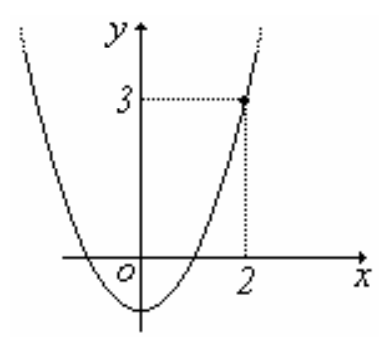
\includegraphics[width=0.5\textwidth]{fig_lim/fig_int_lim}
  \caption{Gráfico da função $f(x)=x^2-1$.}
  \label{fig:func+_x^2-1}
\end{figure}
\end{ex}

Considere agora uma outra função \mat{g(x)=\frac{x^2-1}{x-1}}. Esta função está definida
\mat{\forall x\in\mathbb{R}-\{1\}}. Isto significa que não podemos estabelecer uma imagem quando x assume o valor 1.
\matt{g(1)=\frac{1^2-1}{1-1}=\frac{0}{0}???
}
\mat{\frac{0}{0}} simboliza uma indeterminação\index{indeterminação} matemática. Outros tipos de indeterminações matemáticas serão tratados mais adiante.

Qual o comportamento gráfico da função $g$ quando $x$ assume valores muito próximos de$1$, porém
diferentes de $1$?

A princípio o estudo do limite visa estabelecer o comportamento de uma função numa vizinhança de um ponto (que pode ou não pertencer ao seu domínio). No caso da função $f$, qualquer valor atribuído a $x$ determina uma única imagem, sem problema algum. Mas na função g, existe o ponto $x = 1$ que gera a indeterminação.

Estudemos os valores da função \mat{g(x)=\frac{x^2-1}{x-1}} quando $x$ assume valores próximos
(numa vizinhança) de $1$, mas diferentes de $1$. Para isto vamos utilizar tabelas de aproximações.
\subsection{Tabelas de aproximações}
As tabelas de aproximações são utilizadas para aproximar o valor da imagem de uma
função (se existir) quando a variável $x$ se aproxima de um determinado ponto.
Atribuindo a $x$ valores próximos de $1$, porém \textbf{menores} do que $1$:
\begin{table}[H]
\centering
\begin{tabular}{|c|c|c|c|c|c|c|c|}
\hline
      $x$ & $0$&$ 0,5 $&$0,75 $&$0,9$&$ 0,99$&$ 0,999$&$ 0,9999$\\\hline
      $g(x)$ & $1$& $1,5 $&$1,75 $&$1,9 $&$1,99 $&$1,999 $&$1,9999$\\\hline
    \end{tabular}
    \caption{$x$ tendendo a $1$ pela esquerda}
    \label{tab:xTendendo1Esq}
\end{table}
Atribuindo a $x$ valores próximos de $1$, porém \textbf{maiores} do que $1$:
\begin{table}[H]
\centering
\begin{tabular}{|c|c|c|c|c|c|c|c|}
\hline
      $x$ & $2$&$ 1,5 $&$1,25 $&$1,1$&$ 1,01$&$1,001$&$1,0001$\\\hline
      $g(x)$ & $3$& $2,5 $&$2,25 $&$2,1$&$2,01$&$2,001 $&$2,0001$\\\hline
    \end{tabular}
     \caption{$x$ tendendo a $1$ pela direita}
    \label{tab:xTendendo1Dir}
\end{table}
    Observemos que \textbf{podemos tornar $g(x)$ tão próximo de $2$ quanto desejarmos, bastando
para isso tomarmos $x$ suficientemente próximo de $1$}. De outra forma, dizemos:
\begin{framed}
“O limite da função $g(x)$ quando $x$ se aproxima de (tende a) $1$ é igual a $2$”.
\end{framed}

Simbolicamente escrevemos: \mat{\displaystyle\lim_{x\to 1} g(x)=2} ou \mat{\displaystyle\lim_{x\to 1} \frac{x^2-1}{x-1}=2}

\begin{obs}~
  \begin{compactenum}[1)]
  \item Os dois tipos de aproximações que vemos nas Tabelas \ref{tab:xTendendo1Esq} e \ref{tab:xTendendo1Dir} são chamados de \textbf{limites laterais}.
  \begin{compactenum}[a)]
\item Quando $x$ tende a $1$ por valores menores do que $1$ (Tabela \ref{tab:xTendendo1Esq}), dizemos que $x$ tende a $1$ pela esquerda, e denotamos simbolicamente por $x\to 1^-$ . Temos então que:

\begin{multicols}{2}
\begin{framed}\matt{\lim_{x\to 1^-} g(x)=2 \textrm{ ou } \displaystyle\lim_{x\to 1^-} \frac{x^2-1}{x-1}=2}\end{framed}
\textbf{Atenção:} \textcolor{black!40!red}{ O sinal negativo no expoente do no $1$ simboliza apenas que $x$ se
aproxima do número $1$ pela esquerda.}
\end{multicols}

\item Quando $x$ tende a $1$ por valores maiores do que $1$ (Tabela \ref{tab:xTendendo1Dir}), dizemos que $x$ tende a $1$ pela direita, e denotamos simbolicamente por $x\to 1^+$ . Temos então que:
\begin{multicols}{2}
\begin{framed}\matt{\lim_{x\to 1^+} g(x)=2 \textrm{ ou } \displaystyle\lim_{x\to 1^+} \frac{x^2-1}{x-1}=2}\end{framed}
\textbf{Atenção:} \textcolor{black!40!red}{ O sinal positivo no expoente do no $1$ simboliza apenas que $x$ se
aproxima do número $1$ pela direita.}
\end{multicols}
\end{compactenum}
\item Se a função $g$ se aproximasse de valores distintos à medida que $x$ se aproximasse lateralmente de
\mat{1}, pela esquerda e pela direita, então diríamos que o limite da função $g$ não existiria neste ponto,
simbolicamente  $\displaystyle\nexists \lim_{x\to 1} g(x)=2$
\item  O limite da função $g(x)$ quando $x$ se aproxima de $1$, somente existe se os limites laterais são
iguais. Simbolicamente:
\begin{framed}
 $\displaystyle \lim_{x\to 1} g(x)=2$ se, e somente se, $\displaystyle\lim_{x\to 1^-} g(x)=\lim_{x\to 1^+} g(x)=2$
\end{framed}
  \end{compactenum}
\end{obs}
\textcolor{orange}{Será necessário sempre construir Tabela de aproximações para determinar o limite de uma função,
caso ele exista?}\\
Não! Há uma forma bem mais simples, como veremos mais a frente, tais como fatoração.
\section{Definição de Limite}\hypertarget{ConceitoLimite}{}
Seja $f$ uma função definida em um intervalo aberto em torno de um dado ponto $x_0$, exceto talvez em $x_0$. Quando o valor de $f(x)$ é arbitrariamente próximo de um número $L$ para $x$ suficientemente próximo de $x_0$, escrevemos
\begin{equation*}
  \lim_{x\to x_0} f(x) = L
\end{equation*}
e dizemos que o limite da função $f$ é $L$ quando $x$ tende a $x_0$. Veja a Figura \ref{fig:lim}.

\begin{figure}[H]
  \centering
  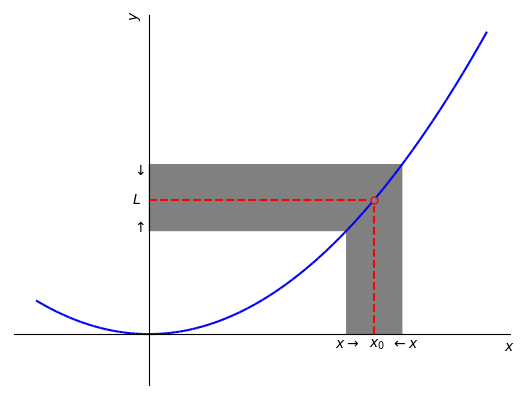
\includegraphics[width=0.6\textwidth]{fig_lim/fig_lim}
  \caption{Ilustração da noção de limite de uma função.}
  \label{fig:lim}
\end{figure}

\begin{ex}\label{ex:lim0}
  Consideremos a função
  \begin{equation*}
    f(x) = \frac{(x^2-1)(x-2)}{(x-1)(x-2)}
  \end{equation*}
  Na Figura \ref{fig:ex_lim0}, temos um esboço do gráfico desta função.

  \begin{figure}[H]
    \centering
    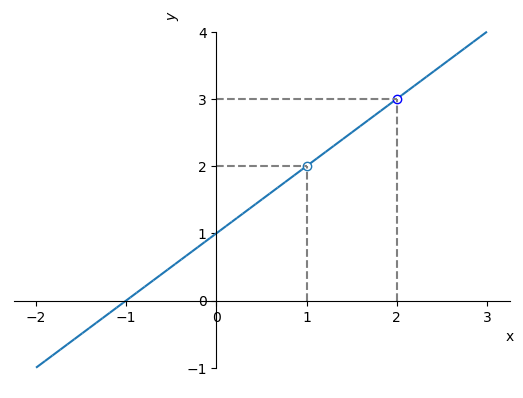
\includegraphics[width=0.6\textwidth]{fig_lim/fig_ex_lim0}
    \caption{Esboço do gráfico da função $f(x)$ dada no Exemplo \ref{ex:lim0}.}
    \label{fig:ex_lim0}
  \end{figure}


  Vejamos os seguintes casos:
  \begin{itemize}
  \item $\displaystyle \lim_{x\to 0} f(x) = 1 = f(0)$.
    
    \begin{tabular}{r|ccc|c|ccc}
      $x$ & $-0,01$ & $-0,001$ & $-0,0001$ & $\rightarrow 0 \leftarrow$ & $0,0001$ & $0,001$ & $0,01$\\\hline
      $f(x)$ & $0,99$ & $0,999$ & $0,9999$ & $\rightarrow 1 \leftarrow$ & $1,0001$ & $1,001$ & $1,01$
    \end{tabular}

    
    No \geogebra, podemos computar este limite com o comando
\begin{verbatim}
limite((x^2-1)*(x-2)/((x-1)*(x-2)),0)
\end{verbatim}
   
  \item $\displaystyle \lim_{x\to 1} f(x) = 2$, embora $f(1)$ não esteja definido.
    
    \begin{tabular}{r|ccc|c|ccc}
      $x$ & $0,9$ & $0,99$ & $0,999$ & $\rightarrow 1 \leftarrow$ & $1,0001$ & $1,001$ & $1,01$\\\hline
      $f(x)$ & $1,9$ & $1,99$ & $1,999$ & $\rightarrow 2 \leftarrow$ & $2,0001$ & $2,001$ & $2,01$
    \end{tabular}
  \item $\displaystyle \lim_{x\to 2} f(x) = 3$, embora $f(2)$ também não esteja definido. Verifique!
  \end{itemize}
\end{ex}

\subsection{Exercícios resolvidos}

\begin{exeresol}
  Estime o valor do limite
  \begin{equation*}
    \lim_{x\to 1} e^x
  \end{equation*}
  \begin{resol}
 Da noção de limite, podemos buscar inferir o limite de uma função em um ponto $x_0$, computando seus valores próximos deste ponto. Por exemplo, construímos a seguinte Tabela:
  
  \begin{tabular}{r|ccc|c|ccc}
    $x$ & $0,9$ & $0,99$ & $0,999$ & $\rightarrow 1 \leftarrow$ & $1,0001$ & $1,001$ & $1,01$\\\hline
    $f(x)$ & $2,460$ & $2,691$ & $2,716$ & $\rightarrow 2,72 \leftarrow$ & $2,719$ & $2,721$ & $2,746$
  \end{tabular}
  
  Com isso, inferimos que
  \begin{equation*}
    \lim_{x\to 1} e^x \approx 2,72
  \end{equation*}
  Mais adiante, veremos que $\lim_{x\to 1} e^x = e \approx 2,718281828459045 ...$
\end{resol}
\end{exeresol}

\begin{exeresol}
  Considere que uma dada função $f$ tenha o seguinte esboço de gráfico:

  \begin{center}
    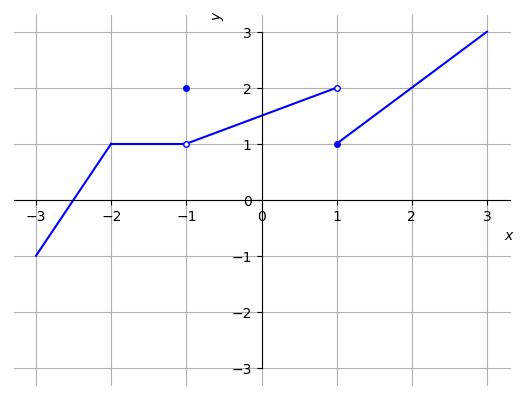
\includegraphics[width=0.6\textwidth]{fig_lim/fig_exeresol_nocaolim}
  \end{center}

  Então, infira o valores de
  \begin{multicols}{3}
  \begin{enumerate}[a)]
  \item $\displaystyle \lim_{x\to -2} f(x)$
  \item $\displaystyle \lim_{x\to -1} f(x)$
  \item $\displaystyle \lim_{x\to 1} f(x)$
  \end{enumerate}\end{multicols}
  \begin{resol}
  \begin{enumerate}[a)]
  \item $\displaystyle \lim_{x\to -2} f(x)$

    Para valores suficientemente próximos de $-2$ e a direita de $-2$ (i.e. $x>-2$), podemos observar que $f(x)=1$. Para tais valores de $x$ a esquerda de $-2$ (i.e. $x<-2$), vemos que os valores de $f(x)$ tornam-se próximos de $1$. Isto é, temos que os valores de $f(x)$ podemos ser tomados arbitrariamente próximos de $L=1$, se tomarmos $x$ suficientemente próximo de $-2$. Concluímos que
    \begin{equation*}
      \lim_{x\to -2} = 1
    \end{equation*}
  \item $\displaystyle \lim_{x\to -1} f(x)$

    Mesmo sendo $f(-1)=2$, observamos que os valores de $f(x)$ podem ser tomados arbitrariamente próximos de $1$, se escolhemos valores de $x$ suficientemente próximos de $-1$. Logo,
    \begin{equation*}
      \lim_{x\to -1} f(x) = 1
    \end{equation*}
    \item $\displaystyle \lim_{x\to 1} f(x)$

      Aqui, para valores de $x$ suficientemente próximos de $x_0=1$ e a esquerda ($x<1$), vemos que os valores de $f(x)$ são próximos de $L=2$. Entretanto, para valores de $x$ suficientemente próximos de $x_0=1$ e a direita ($x>1$), temos que os valores de $f(x)$ são próximos de $L=1$. Ou seja, não é possível escolher um valor $L$ tal que $f(x)$ esteja arbitrariamente próxima ao tomarmos $x$ suficientemente próximo de $x_0=1$, pois $L$ dependerá de $x$ estar a esquerda ou a direita de do ponto $x_0 = 1$. Concluímos que este limite não existe, e escrevemos
      \begin{equation*}
        \not\exists\lim_{x\to 1} f(x)
      \end{equation*}
  \end{enumerate}
\end{resol}
\end{exeresol}

\subsection{Exercícios}
\begin{exer}\label{exer:limgraf}
  Considere que uma dada função $f$ tenha o seguinte esboço de gráfico:
  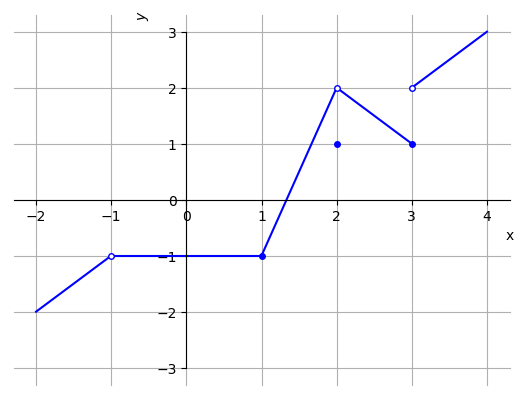
\includegraphics[width=0.5\textwidth]{fig_lim/fig_exer_limgraf}

  Forneça o valor dos seguintes limites:
  \begin{multicols}{2}
    \begin{enumerate}[a)]
  \item $\displaystyle \lim_{x\to -1} f(x)$
  \item $\displaystyle \lim_{x\to 1} f(x)$
  \item $\displaystyle \lim_{x\to 2} f(x)$
  \item $\displaystyle \lim_{x\to 3} f(x)$
  \end{enumerate}\end{multicols}
\end{exer}
\begin{resp}
  a)~$-1$; b)~$-1$; c)~$2$; d)~$\nexists$
\end{resp}

\begin{exer}
  Considerando a mesma função do exercício anterior (Exercício \ref{exer:limgraf}), forneça
  \begin{multicols}{2}
  \begin{enumerate}[a)]
  \item $\displaystyle \lim_{x\to -\frac{3}{2}} f(x)$
  \item $\displaystyle \lim_{x\to 0} f(x)$
  \item $\displaystyle \lim_{x\to \frac{3}{4}} f(x)$
  \end{enumerate}\end{multicols}
\end{exer}
\begin{resp}
  a)~$-\frac{3}{2}$; b)~$-1$; c)~$-1$
\end{resp}

\subsection{Definição formal de limite}
Abaixo, segue uma definição formal de limite.
\begin{framed}
  \begin{definition}~\label{def:DefFormalLimite}
  Seja uma função $f(x)$ definida num intervalo aberto que contém o número $x_0$
(admitimos a possibilidade de que ela não seja definida para ele). Dizemos que 
o limite da função $f(x)$ é $L$ quando $x$ tende a $x_0$, e representamos tal fato por
\matt{
\lim_{x\to x_0} f(x)=L
}
se, e somente se, para todo número $\epsilon > 0$ houver um número $\delta  > 0$ tal que 
 $|f(x)-L|<\epsilon$,  sempre que $0<|x-x_0|<\delta$. 
  \end{definition}
\end{framed}

A Figura \ref{fig:DefFormalLimite} ilustra a Definição \ref{def:DefFormalLimite}. Observe que, quanto menor o valor de $\epsilon$, sempre é possível encontrar um $\delta$ tal que $0<|x-x_0|<\delta$ para $|f(x)-L|<\epsilon$. Vejamos um caso de aplicação da definição acima no exemplo seguinte:
 \begin{figure}[H]
    \centering
    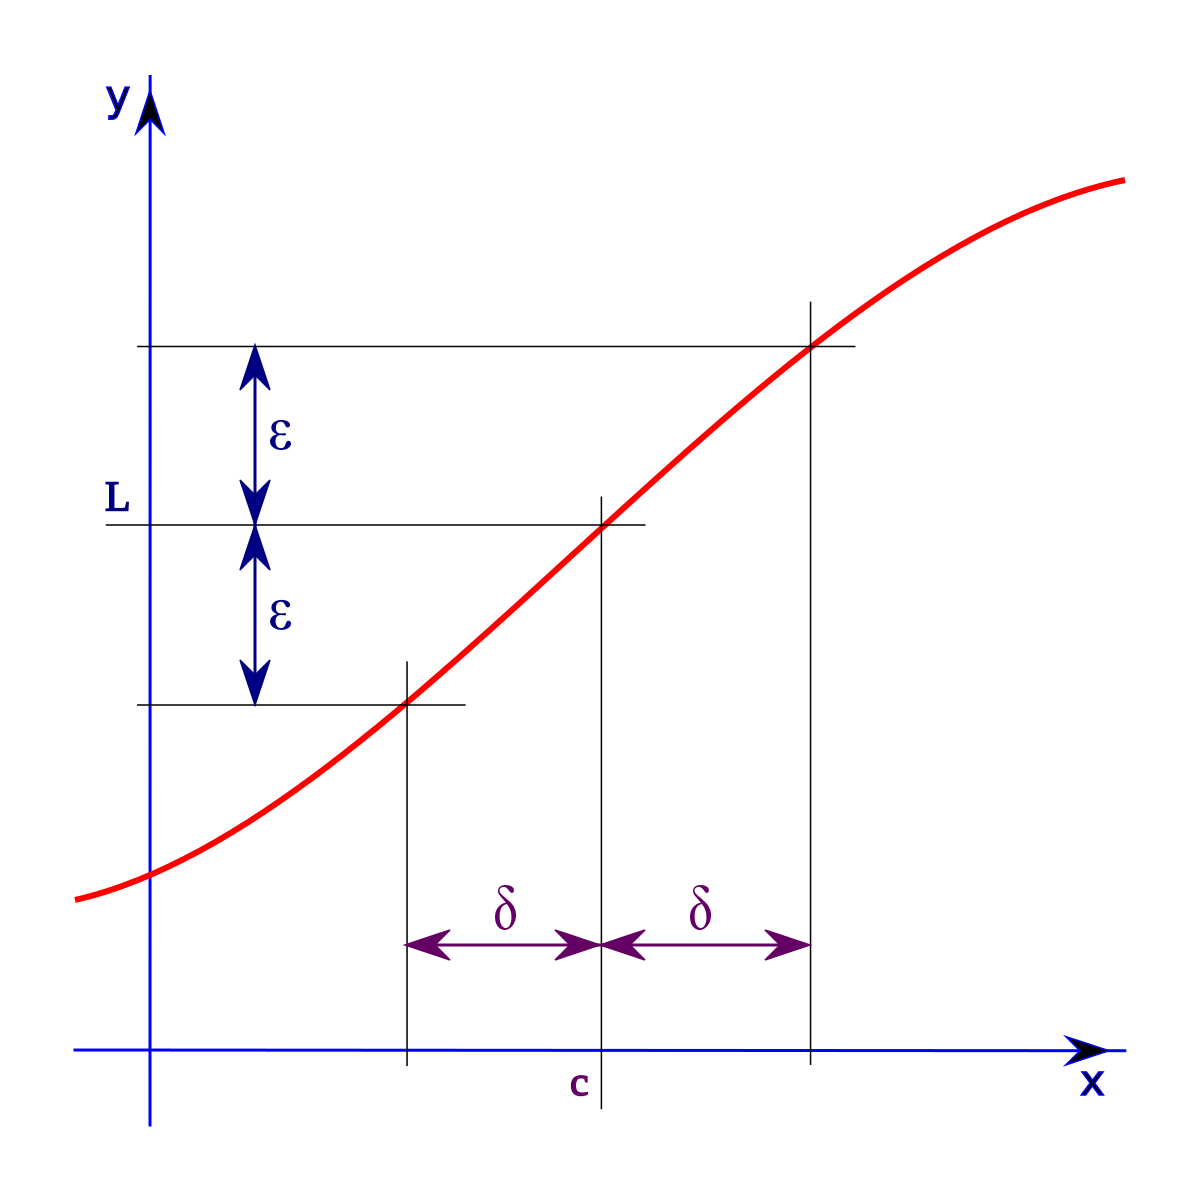
\includegraphics[width=0.45\textwidth]{fig_lim/DefLimiteFormal}
    \caption{Esboço do gráfico da função $f(x)$ dada no Exemplo \ref{ex:lim0}.}
    \label{fig:DefFormalLimite}
  \end{figure}

\vspace{0.1cm}
\begin{ex}
  Vamos utilizar a Definição \ref{def:DefFormalLimite} para mostrar que 
  \matt{
  \lim_{x\to 5} (3x-3)=12
  }
\begin{solution}
  Queremos mostrar que existe um $\delta$ tal que $|(3x-3)-12|<\epsilon$ sempre que $|x-5|<\delta$.
  \matt{
  |(3x-3)-12|<\epsilon\Rightarrow |3x-15|<\epsilon\Rightarrow |3(x-5)|<\epsilon\rightarrow|3||x-5|<\epsilon\Rightarrow |x-5|<\epsilon/3
  }
  que imediatamente dá o resultado desejado se escolhermos
  $$\delta=\epsilon/3$$
\end{solution} 
\end{ex}
\begin{ex}
  Mostre que \matt{
  \lim_{x\to 0} x\sen\pc{\frac{1}{x}}=0
  }
  \begin{solution}
      Nós deixamos que $\epsilon >0$ seja dado. Precisamos encontrar um $ \delta >0$ tal que $|x-0|<\delta$| implica $\left|x\sen\pc{\frac{1}{x}}\right|<\epsilon$

Como a função  seno é limitada entre -1 e 1, temos que $\left|\sen\pc{\frac{1}{x}}\right|<1$. Segue que:
\begin{align*}
    \left|x\sen\pc{\frac{1}{x}}-0\right|&=\left|x\sen\pc{\frac{1}{x}}\right|\\
    &=|x|\left|\sen\pc{\frac{1}{x}}\right|\\
    &\leq |x|
\end{align*}
Assim, se tomarmos $\delta=\epsilon$, então $|x|=|x-0|<\delta $ implica $\left|x\operatorname {sen} \pc{\frac {1}{x}}-0\right|<\epsilon$,  que completa a prova.
  \end{solution}
  
\end{ex}
\nota{
Veremos mais adiante maneiras mais fáceis de calcular limites de funções, em especial funções contínuas.
}

\section{Principais propriedades dos limites}\hypertarget{PropLimite}{}\label{sec:PropLimite}

Sejam dados os seguintes limites
\begin{equation*}
  \lim_{x\to x_0} f(x) = L_1\qquad\text{e}\qquad \lim_{x\to x_0} g(x) = L_2,
\end{equation*}
com $x_0, L_1, L_2, k$ números reais. Então, valem as seguintes Propriedades:
\begin{compactenum}[a)]
\item \textbf{O limite de uma constante é a própria constante}
\begin{equation*}
    \lim_{x\to x_0} k = k
  \end{equation*}
\item \textbf{Propriedade da multiplicação por um escalar:}
  \begin{equation*}
    \lim_{x\to x_0} kf(x) = k\lim_{x\to x_0} f(x) = kL_1,
  \end{equation*}
  para qualquer número real $k$.
\item \textbf{Propriedade da soma/subtração:}
  \begin{equation*}
    \lim_{x\to x_0} f(x) \pm g(x) = \lim_{x\to x_0} f(x) \pm \lim_{x\to x_0} g(x) = L_1 \pm L_2
  \end{equation*}
\item \textbf{Propriedade do produto:}
  \begin{equation*}
    \lim_{x\to x_0} f(x) \cdot g(x) = \lim_{x\to x_0} f(x) \cdot \lim_{x\to x_0} g(x) = L_1 \cdot L_2
  \end{equation*}
\item \textbf{Propriedade do quociente}:
  \begin{equation*}
    \lim_{x\to x_0} \frac{f(x)}{g(x)} = \frac{\lim_{x\to x_0} f(x)}{\lim_{x\to x_0} g(x)} = \frac{L_1}{L_2}
  \end{equation*}
  desde que $L_2\neq 0$.
\item \textbf{Propriedade da potenciação:}
  \begin{equation*}
    \lim_{x\to x_0} (f(x))^n = L_1^n
  \end{equation*}
  se $L_1^s$ é um número real.
  \item \textbf{Limite de uma constante}$$\lim_{x\to x_0} k = k$$
\end{compactenum}

\vspace{0.1cm}
\begin{ex}
  Vejamos os seguintes casos:
  \begin{enumerate}[a)]
  \item $\displaystyle \lim_{x\to -1} 2x$
  \begin{solution}
  \begin{align*}
    \lim_{x\to -1} 2x &= 2\lim_{x\to -1} x\\
    &= 2\cdot(-1) = -2
  \end{align*}

  No \geogebra, podemos computar este limite com
\begin{verbatim}
limite(2*x,-1)
\end{verbatim}
  \end{solution}
  \item $\displaystyle \lim_{x\to 2} x^2 - 1$
  \begin{solution}
  \begin{align*}
    \lim_{x\to 2} x^2 - 1 &= \lim_{x\to 2} x^2 - \lim_{x\to 2} 1\\
                          &= \left(\lim_{x\to 2} x\right)^2 - \lim_{x\to 2} 1\\
    &= 2^2 - 1 = 3
  \end{align*}

  No \geogebra, podemos computar este limite com o comando: \verb+limite(x^2-1,-1)+
  \end{solution}
  \item $\displaystyle \lim_{x\to 0} \sqrt{1-x^2}$.
  \begin{solution}
  \begin{align*}
    \lim_{x\to 0} \sqrt{1-x^2} &= \sqrt{\lim_{x\to 0} 1-x^2}\\
                                &= \sqrt{\lim_{x\to 0} 1 - \left(\lim_{x\to 0} x\right)^2}\\
                                &= \sqrt{1 - (0)^2} \\
                                &= 1
  \end{align*}
  
  No \geogebra, podemos computar este limite com o comando: \verb+limite(sqrt(1-x^2),0)+
  \end{solution}
  
\item $\displaystyle \lim_{x\to 0} \frac{(x^2-1)(x-2)}{(x-1)(x-2)}$
\begin{solution}
    \begin{align*}
    \lim_{x\to 0} \frac{(x^2-1)(x-2)}{(x-1)(x-2)} &= \frac{\displaystyle\lim_{x\to 0}(x^2-1)(x-2)}{\displaystyle\lim_{x\to 0} (x-1)(x-2)}\\
                                                  &= \frac{\displaystyle\lim_{x\to x_0} (x^2-1)\lim_{x\to 0}(x-2)}{\displaystyle\lim_{x\to 0}(x-1)\lim_{x\to 0}(x-2)}\\
    &= \frac{-2}{-2} = 1
  \end{align*}
\end{solution}

  \end{enumerate}
\end{ex}


\subsection{Exercícios}
\begin{exer}
  Calcule os limites abaixo:
  \begin{figure}[H]
  \centering
  \includegraphics[scale=0.4]{fig_lim_exer/CálculoLimitegrupo}
  %\caption{Ilustração da noção de limite lateral à esquerda.}
  %\label{fig:lim_esq}
\end{figure}
\end{exer}
\begin{resp}
\begin{multicols}{3}
\begin{compactenum}[a)]
\item $4$
\item $2/5$
\item $3/5$
\item $3$
\item $-8/3$
\item $1/2$
\item $4/3$
\item $-1/56$
\item $-1/3$
\end{compactenum}
\end{multicols}
 \end{resp}
 
\section{Limites laterais}\hypertarget{LimLateral}{}\label{cap_lim_sec_lateral}
Seja dada uma função $f$ definida para todo $x$ em um intervalo aberto $(a, x_0)$. O {\bf limite lateral à esquerda} de $f$ no ponto $x_0$ é denotado por
\begin{equation*}
  \lim_{x\to x_0^-} f(x)
\end{equation*}
e é computado tendo em vista a tendência da função apenas para pontos $x<x_0$. Em outras palavras, o
\begin{equation*}
  \lim_{x\to x_0^-} f(x) = L
\end{equation*}
quando $f(x)$ pode ser tomado arbitrariamente próximo de $L$, desde que tomemos $x<x_0$ suficientemente próximo de $x_0$. Veja a Figura \ref{fig:lim_esq}.

\begin{figure}[H]
  \centering
  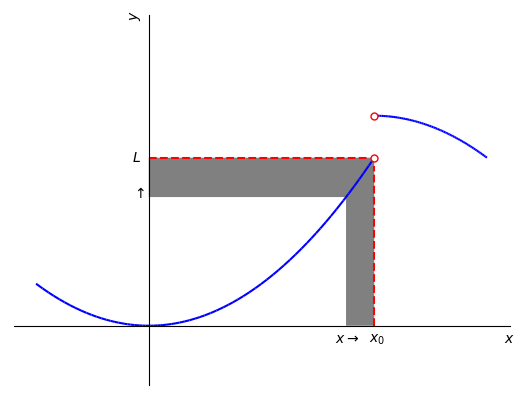
\includegraphics[width=0.7\textwidth]{fig_lim/fig_lim_esq}
  \caption{Ilustração da noção de limite lateral à esquerda.}
  \label{fig:lim_esq}
\end{figure}

Para uma função $f$ definida para todo $x$ em um intervalo aberto $(x_0, b)$, o {\bf limite lateral à direita} de $f$ no ponto $x_0$ é denotado por
\begin{equation*}
  \lim_{x\to x_0^+} f(x)
\end{equation*}
e é computado tendo em vista a tendência da função apenas para pontos $x>x_0$. Em outras palavras, temos
\begin{equation*}
  \lim_{x\to x_0^+} f(x) = L
\end{equation*}
quando $f(x)$ pode ser tomado arbitrariamente próximo de $L$, desde que tomemos $x>x_0$ suficientemente próximo de $x_0$. Veja a Figura \ref{fig:lim_dir}.

\begin{figure}[H]
  \centering
  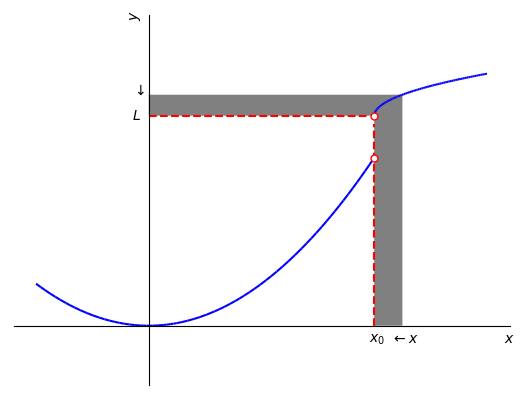
\includegraphics[width=0.58\textwidth]{fig_lim/fig_lim_dir}
  \caption{Ilustração da noção de limite lateral à direita.}
  \label{fig:lim_dir}
\end{figure}

\begin{ex}\label{ex:lim_absx}
  Vamos calcular
  \begin{equation*}
    \lim_{x\to 0^-} |x|.
  \end{equation*}
  \begin{solution}
Por definição, temos
  \begin{equation*}
    |x| = \left\{
      \begin{array}{ll}
        x, & x\geq 0\\
        -x, & x< 0
      \end{array}
    \right.
  \end{equation*}
  Como estamos interessados no limite lateral à esquerda de $x=0$, trabalhamos com $x<0$ e, então
  \begin{equation*}
    \lim_{x\to 0^-} |x| = \lim_{x\to 0^-} -x = -\lim_{x\to 0^-} x = 0
  \end{equation*}
  
  Analogamente, calculamos
  \begin{equation*}
    \lim_{x\to 0^+} |x| = \lim_{x\to 0^+} x = 0
  \end{equation*}
  Verifique!

  
  Usando o \geogebra, podemos computar os limites acima com os seguintes comandos:
  \end{solution}
\end{ex}

\begin{framed}\begin{teo}[Unicidade dos Limites]~\label{teo:lim_existe}
 \\ Existe o limite de uma dada função $f$ no ponto $x=x_0$ e $\displaystyle\lim_{x\to x_0} f(x) = L$ se, e somente se, existem e são iguais a $L$ os limites laterais à esquerda e à direita de $f$ no ponto $x=x_0$.
\end{teo}\end{framed}
\nota{
  O \(\lim\limits_{x \to a} f(x)\) não existe nos seguintes casos:
\begin{itemize}
    \item algum dos limites laterais não existe;

\item os limites laterais existem, porém, são diferentes.
\end{itemize}

Se a função \(f\) é definida por partes para \( x<a\) e para \(x>a\), para encontrar o \(\lim\limits_{x \to a} f(x)\) é necessário calcular os seus respectivos limites laterais.
}
\begin{ex}
  No exemplo anterior (Exemplo \ref{ex:lim_absx}), vimos que
  \begin{equation*}
    \lim_{x\to 0^-} |x| = \lim_{x\to 0^+} |x| = 0
  \end{equation*}
  Logo, pelo teorema acima (Teorema \ref{teo:lim_existe}), podemos concluir que
  \begin{equation*}
    \lim_{x\to 0} |x| = 0
  \end{equation*}
\end{ex}

\begin{ex}
  Vamos verificar a existência de
  \begin{equation*}
    \lim_{x\to 0} \frac{|x|}{x}
  \end{equation*}
  \begin{solution}
      Começamos pelo limite lateral à esquerda, temos
  \begin{align*}
    \lim_{x\to 0^-} \frac{|x|}{x} &= \lim_{x\to 0^-} \frac{-x}{x}\\
    &= \lim_{x\to 0^-} -1 = -1
  \end{align*}
  Agora, calculando o limite lateral à direta, obtemos
  \begin{align*}
    \lim_{x\to 0^+} \frac{|x|}{x} &= \lim_{x\to 0^+} \frac{x}{x}\\
    &= \lim_{x\to 0^+} 1 = 1
  \end{align*}
  Como os limites laterais à esquerda e à direita são diferentes, concluímos que não existe o limite de $|x|/x$ no ponto $x=0$.

    No \geogebra, ao tentar computar o limite com o comando \verb+limite(abs(x)/x,0)+, o resultado dar indefinido. 
  \end{solution}
  \end{ex}
\begin{ex}
  Seja a função \( f\) definida por:

\[f(x)=\left\{\begin{array}{ccl} x^2, & &\mbox{se } x<2; \\ 4 ,& &\mbox{se } x=2; \\ 8-2x, &&\mbox{se } x> 2. \end{array}\right. \]
Calculemos \(\lim\limits_{x \to 2} f(x)\), caso exista.\\\\
\begin{solution}
Como \(f\) tem diferentes regras de correspondência para \( x<2\) e \( x>2\), precisamos calcular os limites laterais:
\begin{itemize}
    \item Limite lateral quando \( x\) tende a \(2\) pela direita, isto é, \( 2<x\):

\[ \lim\limits_{x \to 2^{+}} f(x)= \lim\limits_{x \to 2^{+}}( 8-2x )=8-4=4; \]
\item Limite lateral quando \( x\) tende a \( 2\) pela esquerda, isto é, \( x<2\):

\[ \lim\limits_{x \to 2^{-}} f(x)= \lim\limits_{x \to 2^{-}} x^2 =2^2=4. \]
\end{itemize}
Comparando estes limites laterais, além deles existirem, ambos são iguais. Portanto, o \(\lim\limits_{x \to 2} f(x)\) existe e

\[\lim\limits_{x \to 2} f(x)=4.\]
\end{solution}
\end{ex}
\nota{
  As Propriedades básicas para o cálculo de limites bilaterais que vimos na seção \ref{sec:PropLimite} são estendidas para limites laterais. 
  }
\subsection{Exercícios resolvidos}

\begin{exeresol}
  Considere que uma dada função $f$ tenha o seguinte esboço de gráfico:

  \begin{center}
    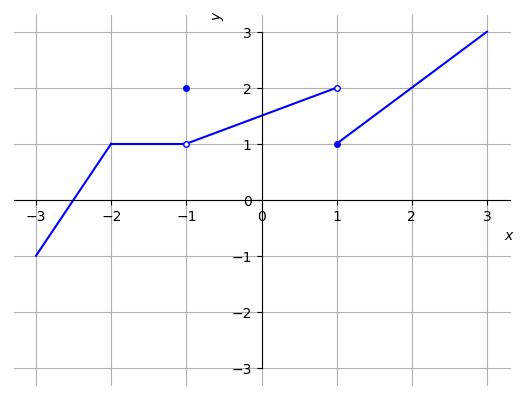
\includegraphics[width=0.7\textwidth]{fig_lim/fig_exeresol_nocaolim}
  \end{center}

  Então, infira o valores de
  \begin{multicols}{3}
  \begin{enumerate}[a)]
  \item $\displaystyle \lim_{x\to -2^-} f(x)$
  \item $\displaystyle \lim_{x\to -1^+} f(x)$
  \item $\displaystyle \lim_{x\to 1^-} f(x)$
  \item $\displaystyle \lim_{x\to 1^+} f(x)$
  \item $\displaystyle \lim_{x\to 1} f(x)$
  \end{enumerate}\end{multicols}
  \begin{resol}~
  \begin{enumerate}[a)]
  \item $\displaystyle \lim_{x\to -2^-} f(x)$

    Para valores $x<-2$ e suficientemente próximos de $-2$, podemos observar que $f(x)$ fica arbitrariamente próximo de $1$. Concluímos que
    \begin{equation*}
      \lim_{x\to -2^-} = 1
    \end{equation*}

  \item $\displaystyle \lim_{x\to -1^+} f(x)$

    Mesmo sendo $f(-1)=2$, observamos que os valores de $f(x)$ podem ser tomados arbitrariamente próximos de $1$, se escolhemos valores de $x>-1$ e suficientemente próximos de $-1$. Logo,
    \begin{equation*}
      \lim_{x\to -1^+} f(x) = 1
    \end{equation*}

  \item $\displaystyle \lim_{x\to 1^-} f(x)$

    Observamos que os valores de $f(x)$ podem ser tomados arbitrariamente próximos de $2$, se escolhemos valores de $x<1$ e suficientemente próximos de $1$. Logo,
    \begin{equation*}
      \lim_{x\to 1^-} f(x) = 2
    \end{equation*}
    Notamos também que, neste caso, $f(x)$ não tende para $f(1)=1$ quando $x$ tende a $1$ pela esquerda.

  \item $\displaystyle \lim_{x\to 1^+} f(x)$

    Observamos que os valores de $f(x)$ podem ser tomados arbitrariamente próximos de $1$, se escolhemos valores de $x>1$ e suficientemente próximos de $1$. Logo,
    \begin{equation*}
      \lim_{x\to 1^+} f(x) = 1
    \end{equation*}
    Aqui, $f(x)\to f(1)=1$ quando $x\to 1^+$.

    \item $\displaystyle \lim_{x\to 1} f(x)$

      Nos itens anteriores, vimos que
      \begin{equation*}
        2 = \lim_{x\to 1^-} f(x) \neq \lim_{x\to 1^+} f(x) = 1
      \end{equation*}
      Logo, concluímos que este limite não existe, e escrevemos
      \begin{equation*}
        \not\exists\lim_{x\to 1} f(x)
      \end{equation*}
  \end{enumerate}
\end{resol}
\end{exeresol}


\begin{exeresol}
  Calcule $\displaystyle\lim_{x\to -1} f(x)$ para
  \begin{equation*}
    f(x) = \left\{
      \begin{array}{ll}
        (x+1)^2-1, & x<-1,\\
        x, & x>-1
      \end{array}
\right.
  \end{equation*}
  \begin{resol}
  A função $f$ tem comportamentos distintos para valores à esquerda e à direita de $x_0=-1$. Portanto, para calcularmos $\displaystyle\lim_{x\to -1} f(x)$ precisamos calcular os limites laterais. Temos:
  \begin{align*}
    \lim_{x\to -1^-} f(x) &= \lim_{x\to -1^-} (x+1)^2-1\\
                          &= (-1+1)^2-1 = -1
  \end{align*}
  e
  \begin{align*}
    \lim_{x\to -1^+} f(x) &= \lim_{x\to -1^+} x\\
                          &= -1
  \end{align*}
  Como ambos os limites laterais são iguais a $-1$, concluímos que
  \begin{equation*}
    \lim_{x\to -1} f(x) = -1
  \end{equation*}
\end{resol}
\end{exeresol}

\begin{exeresol}
  Seja a função \( f\) definida por:

\[ f(x)=x\sqrt{\dfrac{1}{4x^2}-16} \]
Calculemos \(\lim\limits_{x \to 0} f(x)\), caso exista.\\
\begin{resol}
  Analisando \(f\), temos que

\[ f(x)= x\sqrt{\dfrac{1}{4x^2}-16} = x\sqrt{\dfrac{1-64x^2}{4x^2}} = \dfrac{x\sqrt{1-64x^2}}{2|x|}. \]
Logo, \(f\) pode ser reescrita por partes em \( 0\) :

\[f(x)=\left\{\begin{array}{ccl} -\dfrac{\sqrt{1-64x^2}}{2}, & &\mbox{se } x<0; \\ \dfrac{\sqrt{1-64x^2}}{2}, & &\mbox{se } x\geq 0 . \end{array}\right. \]
Então, para calcular \(\lim\limits_{x \to 0} f(x)\), precisamos calcular os limites laterais:
\begin{itemize}
    \item Limite lateral quando \( x\) tende a \(0\) pela esquerda, isto é, \(x<0\):

\[ \lim\limits_{x \to 0^{-}} -\dfrac{\sqrt{1-64x^2}}{2}= -\dfrac{1}{2}; \]
\item Limite lateral quando \( x\) tende a \(0\) pela direita, isto é, \( x>0\):

\[ \lim\limits_{x \to 0^{+}} \dfrac{\sqrt{1-64x^2}}{2}=\dfrac{1}{2}. \]
\end{itemize}

Comparando estes limites laterais, observamos que embora eles existam, não são iguais. Portanto, o \(\lim\limits_{x \to 2} f(x)\) não existe.
\end{resol}
\end{exeresol}
\subsection{Exercícios}

\begin{exer}\label{exer:limgraf_lat}
  Considere que uma dada função $f$ tenha o seguinte esboço de gráfico:

  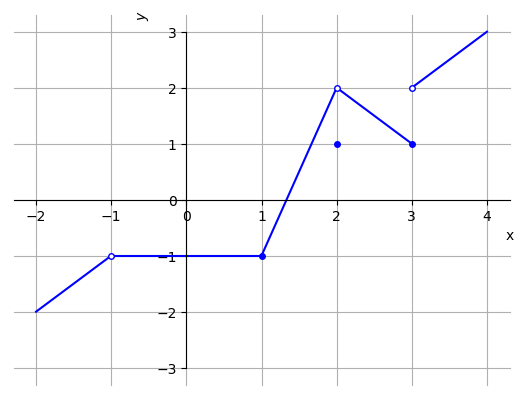
\includegraphics[width=0.55\textwidth]{fig_lim/fig_exer_limgraf}

  Forneça o valor dos seguintes limites:
  \begin{multicols}{3}
  \begin{enumerate}[a)]
  \item $\displaystyle \lim_{x\to 2^+} f(x)$
  \item $\displaystyle \lim_{x\to 2^-} f(x)$
  \item $\displaystyle \lim_{x\to 2} f(x)$
  \item $\displaystyle \lim_{x\to 3^+} f(x)$
  \item $\displaystyle \lim_{x\to 3^-} f(x)$
  \item $\displaystyle \lim_{x\to 3} f(x)$
  \end{enumerate}
  \end{multicols}
\end{exer}
\begin{resp}
  a)~$2$; b)~$2$; c)~$2$; d)~$2$; e)~$1$; f)~$\nexists$
\end{resp}

\begin{exer}
  Sendo
  \begin{equation*}
    f(x) = \left\{
      \begin{array}{ll}
        x^2+1, & x\leq 1\\
        2x, & x>1
      \end{array}
    \right.
  \end{equation*}
  calcule
  \begin{multicols}{3}
  \begin{enumerate}[a)]
  \item $\displaystyle \lim_{x\to 1^-} f(x)$
  \item $\displaystyle \lim_{x\to 1^+} f(x)$
  \item $\displaystyle \lim_{x\to 1} f(x)$
  \end{enumerate}\end{multicols}
\end{exer}
\begin{resp}
  a)~$2$; b)~$2$; c)~$2$
\end{resp}

\begin{exer}
  Sendo
  \begin{equation*}
    f(x) = \left\{
      \begin{array}{ll}
        x^2+1 &, x\leq 1\\
        2x+1 &, x>1
      \end{array}
    \right.
  \end{equation*}
  calcule
  \begin{multicols}{3}
  \begin{enumerate}[a)]
  \item $\displaystyle \lim_{x\to 1^-} f(x)$
  \item $\displaystyle \lim_{x\to 1^+} f(x)$
  \item $\displaystyle \lim_{x\to 1} f(x)$
  \end{enumerate}\end{multicols}
\end{exer}
\begin{resp}
  a)~$2$; b)~$3$; c)~$\nexists$
\end{resp}

\begin{exer}
  Calcule
  \begin{equation*}
    \lim_{x\to 0^-} \frac{x}{2|x|}
  \end{equation*}
\end{exer}
\begin{resp}
  $-\frac{1}{2}$
\end{resp}

\begin{exer}
  Calcule
  \begin{equation*}
    \lim_{x\to -1^+} \sqrt{1-x^2}
  \end{equation*}
  O que pode-se dizer sobre o limite à esquerda?
\end{exer}
\begin{resp}
  $0$; Não está definido, pois o domínio de $f(x)=\sqrt{1-x^2}$ é $[-1, 1]$.
\end{resp}

\section{Cálculo de  indeterminação do tipo 0/0}\hypertarget{Ind0/0}{}
Quando $\displaystyle \lim_{x\to a} f(a)=0$ e $\displaystyle \lim_{x\to a} g(a)=0$, dizemos que
\begin{equation*}
  \lim_{x\to a} \frac{f(x)}{g(x)}
\end{equation*}
é uma {\bf indeterminação do tipo $0/0$}. Deveremos \textbf{simplificar}\footnote{ Para simplificar a expressão você deve utilizar fatoração, racionalização, dispositivo prático de Briot-Ruffini para dividir polinômios, etc \ldots }  a  expressão da função envolvida. Logo após, calculamos o limite da função substituindo, na  expressão já simplificada, o valor de $x$. Em vários destes casos, podemos calcular o limite eliminando o fator em comum $(x-a)$.\\


\begin{ex}
  \begin{align*}
    \lim_{x\to 2}\frac{(x^2-1)(x-2)}{(x-1)(x-2)} = \lim_{x\to 2} \frac{x^2-1}{x-1} = 3
  \end{align*}
  
  No \geogebra~podemos computar o limite acima com o comando:\\ \verb|limite((x**2-1)*(x-2)/((x-1)*(x-2)),2)|
\end{ex}

\nota{
Quando o fator em comum não aparece explicitamente, podemos tentar trabalhar algebricamente de forma a explicitá-lo.
}
\begin{ex}
  No caso do limite
  \begin{align*}
    \lim_{x\to 1} \frac{x^3-3x^2-x+3}{x^2+x-2}
  \end{align*}
  temos que o denominador $p(x) = x^3-3x^2-x+3$ se anula em $x=1$, assim como o denominador $q(x) = x^2+x-2$. Assim sendo, $(x-1)$ é um fator comum entre $p(x)$ e $q(x)$. Para explicitá-lo, 
  \begin{equation*}
    \frac{p(x)}{x-1} = x^2-2x-3\qquad\text{e}\qquad\frac{q(x)}{x-1} = x+2
  \end{equation*}
  
  No \geogebra, podemos computar estas divisões com os seguintes comandos:
\begin{verbatim}
simplify((x**3-3*x**2-x+3)/(x-1))
simplify((x**2+x-2)/(x-1))
\end{verbatim}
 
  Realizadas as divisões, temos
  \begin{equation*}
    p(x) = (x-1)(x^2-2x-3)\qquad\text{e}\qquad q(x)=(x-1)(x+2)
  \end{equation*}
  Com isso, temos
  \begin{align*}
    \lim_{x\to 1} \frac{x^3-3x^2-x+3}{x^2+x-2} &= \lim_{x\to 1} \frac{(x-1)(x^2-2x-3)}{(x-1)(x+2)} \\
    &- \lim_{x\to 1} \frac{x^2-2x-3}{x+2} = -\frac{4}{3}
  \end{align*}
\end{ex}

\begin{ex}
  Calcule
  \begin{equation*}
    \lim_{x\to 0} \frac{\sqrt{1-x}-1}{x}
  \end{equation*}
  \begin{solution}
    Neste caso temos uma indeterminação do tipo $0/0$ envolvendo uma raiz. Neste caso, podemos calcular o limite usando de racionalização
  \begin{align*}
    \lim_{x\to 0} \frac{\sqrt{1-x}-1}{x} &= \lim_{x\to 0} \frac{\sqrt{1-x}-1}{x}\frac{\sqrt{1-x}+1}{\sqrt{1-x}+1}\\
                                         &= \lim_{x\to 0} \frac{1-x-1}{x(\sqrt{1-x}+1)} \\
                                         &= \lim_{x\to 0} \frac{-x}{x(\sqrt{1-x}+1)}\\
    &= \lim_{x\to 0} \frac{-1}{\sqrt{1-x}+1} = -\frac{1}{2}
  \end{align*}
  
  Com o \geogebra, podemos computar este limite com \verb+limit((sqrt(1-x)-1)/x,x,0)+ ou simplesmente com 
\verb+limite((sqrt(1-x)-1)/x,0)+.
  \end{solution}
 \end{ex}

\subsection{Exercícios resolvidos}

\begin{exeresol}
  Calcule
  \begin{equation*}
    \lim_{x\to -1} \frac{x - x^2}{\sqrt{x^2+3}}
  \end{equation*}
  \begin{resol}
  Usando das propriedades de limites, calculamos
  \begin{align*}
    \lim_{x\to -1} \frac{x-x^2}{\sqrt{x^2+3}} &= \frac{\displaystyle\lim_{x\to -1} x-x^2}{\displaystyle\lim_{x\to -1} \sqrt{x^2+3}} \\
                                              &= \frac{-1-(-1)^2}{\sqrt{\displaystyle\lim_{x\to -1} x^2+3}} \\
                                              &= \frac{-2}{\sqrt{4}} \\
                                              &= -1
  \end{align*}
\end{resol}
\end{exeresol}


\begin{exeresol}
  Assumindo que o $\displaystyle\lim_{x\to 2} f(x) = L$ e que
  \begin{equation*}
    \lim_{x\to 2} \frac{f(x)-2}{x+2} = 1,
  \end{equation*}
  forneça o valor de $L$.\\
  \begin{resol}
  Das propriedades de limites, temos
  \begin{align*}
    \lim_{x\to 2} \frac{f(x)-2}{x+2} = 1 &\Rightarrow \frac{\lim_{x\to 2} f(x)-2}{\lim_{x\to 2} x+2} = 1\\
                                         &\Rightarrow \frac{\lim_{x\to 2} f(x) - \lim_{x\to 2} 2}{2+2} = 1\\
                                         &\Rightarrow \frac{L-2}{4} = 1\\
                                         &\Rightarrow L-2 = 4\\
                                         &\Rightarrow L = 6
  \end{align*}
\end{resol}
  \end{exeresol}

\begin{exeresol}
  Calcule
  \begin{equation*}
    \lim_{x\to -1} \frac{x+1}{2-\sqrt{x^2+3}}
  \end{equation*}
  \begin{resol}
  Neste caso, não podemos usar a Propriedade do quociente, pois
  \begin{equation*}
    \lim_{x\to -1} 2-\sqrt{x^2+3} = 0
  \end{equation*}
  Agora, como também temos
  \begin{equation*}
    \lim_{x\to -1} x+1 = 0,
  \end{equation*}
  concluímos se tratar de uma indeterminação $0/0$. Por racionalização, obtemos
  \begin{align*}
    \lim_{x\to -1} \frac{x+1}{2-\sqrt{x^2+3}} &= \lim_{x\to -1} \frac{x+1}{2-\sqrt{x^2+3}}\frac{2+\sqrt{x^2+3}}{2+\sqrt{x^2+3}} \\
                                              &= \lim_{x\to -1} \frac{(x+1)(2+\sqrt{x^2+3})}{4 - (x^2+3)}\\
                                              &= \lim_{x\to -1} \frac{(x+1)(2+\sqrt{x^2+3})}{1-x^2}\\
                                              &= \lim_{x\to -1} \frac{(x+1)(2+\sqrt{x^2+3})}{(1+x)(1-x)}\\
                                              &= \lim_{x\to -1} \frac{2+\sqrt{x^2+3}}{1-x} \\
                                              &= \frac{4}{2} = 2
  \end{align*}
\end{resol}
\end{exeresol}


\begin{exeresol}
  Calculemos os seguintes limites:
\begin{compactenum}[a)]
\item \( \lim\limits_{x \to -4} \frac{x^2-16}{3x+12}\)\\
\begin{resol}
Ao analisar o numerador e o denominador desse quociente, observamos que temos uma indeterminação da forma \(\frac{0}{0}\), pois \( \lim\limits_{x \to -4} (x^2-16)=0\) e \( \lim\limits_{x \to -4} (3x+12)=0\).

Porém, observamos que o termo \((x+4)\) pode ser fatorado de cada um deles, pois

\[ x^2-16=(x+4)(x-4)\quad \mbox{e } \quad 3x+12=3(x+4). \]
Logo,

\[ \lim\limits_{x \to -4} \dfrac{x^2-16}{3x+12} =\lim\limits_{x \to -4} \dfrac{\cancel{(x+4)}(x-4)}{3\cancel{(x+4)}} = \lim\limits_{x \to -4} \dfrac{x-4}{3}= \dfrac{1}{3}\lim\limits_{x \to -4} (x-4)=\dfrac{1}{3}(8)=-\dfrac{8}{3}\]
\end{resol}
\item \( \lim\limits_{x \to 0} \dfrac{\sqrt{x+3}-\sqrt{3}}{x}\)\\
\begin{resol}
Da mesma forma que o item acima, esse limite tem uma indeterminação da forma \(\dfrac{0}{0}\). Para resolver tal problema, precisamos racionalizar o numerador, isto é, multiplicar tanto o numerador quanto o denominador por \( \sqrt{x+3}+\sqrt{3}\):
\[ \lim\limits_{x \to 0} \dfrac{\sqrt{x+3}-\sqrt{3}}{x} = \lim\limits_{x \to 0}\dfrac{(\sqrt{x+3}-\sqrt{3})(\sqrt{x+3}+\sqrt{3})}{x(\sqrt{x+3}+\sqrt{3})}=\lim\limits_{x \to 0} \dfrac{x+3-3}{x(\sqrt{x+3}+\sqrt{3})} = \] \[ \lim\limits_{x \to 0} \dfrac{\cancel{x}}{\cancel{x}(\sqrt{x+3}+\sqrt{3})} = \lim\limits_{x \to 0} \dfrac{1}{\sqrt{x+3}+\sqrt{3}}= \dfrac{1}{\sqrt{3}+\sqrt{3}}= \dfrac{1}{2\sqrt{3}}. \]
\end{resol}
\end{compactenum}
\end{exeresol}
\nota{
  Para racionalizar, precisamos lembrar que:
\[ \begin{array}{lcr} (a^n-b^n)&=&(a-b)\underbrace{(a^{n-1}+a^{n-2}b+a^{n-3}b^2+\ldots+ab^{n-2}+b^{n-1})}_{\mbox{{\bf fator racionalizante}}}\\ (a^n+b^n)&=&(a+b)\overbrace{(a^{n-1}-a^{n-2}b+a^{n-3}b^2-\ldots-ab^{n-2}+b^{n-1})}^{ } \end{array} \]
}
\begin{exeresol}
  Calculemos os seguintes limites:
\begin{compactenum}[a)]
\item \( \lim\limits_{x \to 4} \frac{3-\sqrt{5+x}}{1-\sqrt{5-x}}\)
\begin{resol}
Esse limite tem uma indeterminação da forma \(\dfrac{0}{0}\), nesse caso, devemos fazer uma dupla racionalização:

\[ \begin{array}{rcl} \lim\limits_{x \to 4} \dfrac{3-\sqrt{5+x}}{1-\sqrt{5-x}}& = & \lim\limits_{x \to 4} \dfrac{(3-\sqrt{5+x})(3+\sqrt{5+x}) (1+\sqrt{5-x})}{(1-\sqrt{5-x})(1+\sqrt{5-x})(3+\sqrt{5+x})}\\ \\ & =& \lim\limits_{x \to 4}\dfrac{-\cancel{(x-4)}(1+\sqrt{5-x})}{(3+\sqrt{5+x})\cancel{(x-4)}}= -\lim\limits_{x \to 4}\dfrac{1+\sqrt{5-x}}{3+\sqrt{5+x}} \\ \\ &=& -\dfrac{1+1}{3+3}=-\dfrac{2}{6}= -\dfrac{1}{3}. \end{array} \]
\end{resol}
\item \( \lim\limits_{x \to 0} \dfrac{\sqrt{1+x^2}-\sqrt[4]{1+x^4}}{x^2}\)
\begin{resol}
Aqui temos a indeterminação da forma \(\dfrac{0}{0}\), e observamos que

\[ \begin{array}{l} \sqrt{1+x^2}-\sqrt[4]{1+x^4}=\sqrt[4]{(1+x^2)^2}-\sqrt[4]{1+x^4}=\\ \\ = \dfrac{(1+x^2)^2 -(1+x^4)}{\sqrt{(1+x^2)^3} +(1+x^2)\sqrt[4]{1+x^4} + \sqrt{1+x^2}\sqrt{1+x^4} + \sqrt[4]{(1+x^4)^3}}=\\ \\ = \dfrac{2x^2}{\sqrt{(1+x^2)^3} +(1+x^2)\sqrt[4]{1+x^4} + \sqrt{1+x^2}\sqrt{1+x^4} + \sqrt[4]{(1+x^4)^3}}. \end{array} \]
Logo, calcular o limite acima é equivalente a calcular

\[ \lim\limits_{x\to 0}\dfrac{2\cancel{x^2}}{\cancel{x^2}\left[\sqrt{(1+x^2)^3} +(1+x^2)\sqrt[4]{1+x^4} + \sqrt{1+x^2}\sqrt{1+x^4} + \sqrt[4]{(1+x^4)^3}\right]} = \] \[ \lim\limits_{x\to 0}\dfrac{2}{\left[\sqrt{(1+x^2)^3} +(1+x^2)\sqrt[4]{1+x^4} + \sqrt{1+x^2}\sqrt{1+x^4} + \sqrt[4]{(1+x^4)^3}\right]}=\]\\
\[= \dfrac{2}{1+1+1+1}=\dfrac{1}{2}. \]
Portanto,

\[ \lim\limits_{x \to 0} \dfrac{\sqrt{1+x^2}-\sqrt[4]{1+x^4}}{x^2} =\dfrac{1}{2}. \]
\end{resol}
\item \( \lim\limits_{x \to 64} \dfrac{\sqrt{x}-8}{\sqrt[3]{x}-4}\)\\
\begin{resol}
Assim como nos casos anteriores, a indeterminação é da forma \(\dfrac{0}{0}\) e poderíamos fazer uma dupla racionalização, porém, os cálculos se tornariam muito complicados. Por outro lado, observando as quantidades sub-radicais, notamos que elas são iguais, o que será útil se fizermos uma mudança de variável com o intuito de simplificar a expressão.

Escolhe-se uma variável que seja igual à quantidade sub-radical e o expoente desta variável é o mínimo múltiplo comum dos índices dos radicais. Em nosso caso, como \( {\rm m.m.c}(2,3)=6\) fazemos \(y^6=x\), notemos que \(x\to 64\) implica que \(y\to 2\), e quando substituímos no limite acima, obtemos:
\begin{align*}
    \lim\limits_{x \to 64} \dfrac{\sqrt{x}-8}{\sqrt[3]{x}-4}= \lim\limits_{y\rightarrow 2} \dfrac{y^3-8}{y^2-4}
     &=\lim\limits_{y \to 2} \dfrac{\cancel{(y-2)}(y^2+2y+4)}{\cancel{(y-2)}(y+2)}\\&= \lim\limits_{y \to 2} \dfrac{y^2+2y+4}{y+2}= \dfrac{4+4+4}{2+2}=3
\end{align*}
\end{resol}
\end{compactenum}

\end{exeresol}
\subsection{Exercícios}

\begin{exer}
  Sabendo que $\displaystyle    \lim_{x\to 2} f(x) = 2$,   calcule:
  \begin{multicols}{3}
   \begin{enumerate}[a)]
  \item $\displaystyle \lim_{x\to 2} 2\cdot f(x)$
  \item $\displaystyle \lim_{x\to 2} \pi\cdot f(x)$
  \item $\displaystyle \lim_{x\to 2} -e^{\sqrt{2}}\cdot f(x)$
  \end{enumerate}
  \end{multicols}
 \end{exer}
\begin{resp}
  a)~$2$; b)~$2\pi$; c)~$-2e^{\sqrt{2}}$
\end{resp}

\begin{exer}
  Considerando que
  \begin{equation*}
    \lim_{x\to 3} f(x) = -2\quad\text{e}\quad\lim_{x\to 3} g(x) = \frac{1}{2}
  \end{equation*}
  calcule:
  \begin{enumerate}[a)]
  \item $\displaystyle\lim_{x\to 3} [f(x)+g(x)]$
  \item $\displaystyle\lim_{x\to 3} [g(x)-f(x)]$
  \item $\displaystyle\lim_{x\to 3} [f(x)-2g(x)]$
  \end{enumerate}
\end{exer}
\begin{resp}
  a)~$-3/2$; b)~$5/2$; c)~$-3$
\end{resp}

\begin{exer}
  Considerando que
  \begin{equation*}
    \lim_{x\to 0} f(x) = 3\quad\text{e}\quad\lim_{x\to 0} g(x) = -2,
  \end{equation*}
  calcule:
  \begin{enumerate}[a)]
  \item $\displaystyle\lim_{x\to 0} \pr{f(x)\cdot g(x)}$
  \item $\displaystyle\lim_{x\to 0} \pr{g(x)\cdot (\frac{1}{2}\cdot f(x))}$
  \end{enumerate}
\end{exer}
\begin{resp}
  a)~$-6$; b)~$-3$;
\end{resp}

\begin{exer}
  Considerando que
  \begin{equation*}
    \lim_{x\to 0} f(x) = -2\quad\text{e}\quad\lim_{x\to 0} g(x) = -3,
  \end{equation*}
  calcule:
  \begin{multicols}{2}
    \begin{enumerate}[a)]
  \item $\displaystyle\lim_{x\to 0} \frac{f(x)}{g(x)}$
  \item $\displaystyle\lim_{x\to 0} \frac{g(x)}{2f(x)}$
  \end{enumerate}
  \end{multicols}
\end{exer}
\begin{resp}
  a)~$2/3$; b)~$3/4$;
\end{resp}

\begin{exer}
  Considerando que
  \begin{equation*}
    \lim_{x\to -1} f(x) = -1\quad\text{e}\quad\lim_{x\to -1} g(x) = 4,
  \end{equation*}
  calcule:
  \begin{multicols}{3}
    \begin{enumerate}[a)]
  \item $\displaystyle\lim_{x\to -1} \sqrt{g(x)}$
  \item $\displaystyle\lim_{x\to -1} \sqrt[3]{f(x)}$
  \item $\displaystyle\lim_{x\to -1} (f(x))^{\frac{4}{3}}$
  \end{enumerate}
  \end{multicols}

\end{exer}
\begin{resp}
  a)~$2$; b)~$-1$; c)~$1$
\end{resp}

\begin{exer}
  Calcule os limites:
  \begin{enumerate}[a)]
  \item $\displaystyle\lim_{x\to -2} -3x$\\
  \item $\displaystyle\lim_{x\to -2} x^2-3x$\\    
  \item $\displaystyle\lim_{x\to -2} x^2-3x+\sqrt{x^2}$\\    
  \end{enumerate}
\end{exer}
\begin{resp}
  a)~$6$; b)~$10$; c)~$12$
\end{resp}

\begin{exer}
  Calcule os limites:
  \begin{multicols}{2}
  \begin{enumerate}[a)]
  \item $\displaystyle\lim_{x\to -1} \frac{x}{x-1}$\\
  \item $\displaystyle\lim_{x\to -1} \frac{x^2+x-2}{x^2-3x+2}$\\    
  \end{enumerate}
  \end{multicols}
\end{exer}
\begin{resp}
  a)~$1/2$; b)~$-1/3$;
\end{resp}

\begin{exer}
  Calcule o limite
  \begin{equation*}
    \lim_{x\to 6} \frac{2-\sqrt{x-2}}{x-6}
  \end{equation*}
\end{exer}
\begin{resp}
  $-1/4$
\end{resp}

\section{Limite fundamental exponencial}\hypertarget{LimFundExp}{}
O número $e$ tem grande importância em diversos ramos das ciências, pois está presente 
em vários fenômenos naturais, por exemplo: Crescimento populacional, crescimento de populações 
de bactérias, desintegração radioativa (datação por carbono), circuitos elétricos, etc. Na área de 
economia, é aplicado no cálculo de juros. 

 Foi o Matemático Inglês Jonh Napier (1550-1617) o responsável pelo desenvolvimento 
da teoria logarítmica utilizando o número $e$ como base. O número $e$ é irracional, ou seja, não pode 
ser escrito sob forma de fração, e vale aproximadamente: 
\begin{center}
    \textbf{\textcolor{red}{$e\approx 2,7182818$}}
\end{center}
Como o número $e$ é encontrado em diversos fenômenos naturais, a função exponencial \mat{f(x)=e^x} é considerada uma das funções mais importantes da matemática, merecendo atenção especial de cientistas de diferentes áreas do conhecimento humano. 
\begin{framed}
  \begin{prop}
  \matt{\lim_{x\to +\infty}\pc{1+\frac{1}{x}}^x=e}
  \end{prop}
\end{framed}
A prova desta proposição envolve noções de séries. Utilizaremos o recurso das tabelas de 
aproximações e gráfico para visualizar este resultado. 
\renewcommand{\arraystretch}{2}%Aumenta o espaçamento entre linhas de uma tabela (o número é que define o tamanho do espaçamento
\begin{table}[htb]
    \centering
    \begin{tabular}{|c|c|}
    \hline
         x &  \mat{\displaystyle\lim_{x\to +\infty}\pc{1+\frac{1}{x}}^x=e}\\[0.5ex]\hline 
      1   & 2\\\hline
      2 & 2,25\\\hline
      \vdots &\vdots\\\hline
      10 &2,5993\ldots\\\hline
        \vdots &\vdots\\\hline
        100 & 2,7048\ldots\\\hline
          \vdots &\vdots\\\hline
          1000 & 2,7169\ldots\\\hline
            \vdots &\vdots\\\hline
            100000 & 2,7182\ldots\\\hline
    \end{tabular}
    \caption{Aproximações para \mat{\displaystyle\lim_{x\to +\infty}\pc{1+\frac{1}{x}}^x} quando $x$ tende a $\infty$}
    \label{tab:funcE}
\end{table}
Faça uma tabela para $x\to -\infty$. Abaixo um esboço do gráfico. 
\begin{figure}[htb]
    \centering
     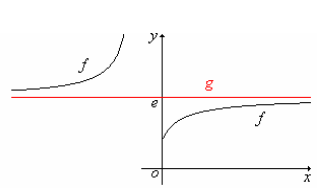
\includegraphics[width=0.6\textwidth]{fig_lim/AproxFuncE}
  \caption{Representação das funções \mat{\displaystyle\lim_{x\to +\infty}\pc{1+\frac{1}{x}}^x} e \ $g(x)=e$}
  \label{fig:LimFuncE}
\end{figure}

\textbf{Consequências importantes do limite fundamental exponencial:}\\
 (i) \mat{\displaystyle\lim_{x\to 0}\pc{1+x}^{\frac{1}{x}}=e}\hfill (ii) \mat{\displaystyle\lim_{x\to 0} \frac{a^x-1}{x}=\ln (a), a>0, \forall a\neq 1}

\section{Limite fundamental trigonométrico}\hypertarget{LimFundTrig}{}\label{sec:LimFundTrig}
O limite fundamental trigonométrico trata de um limite cuja indeterminação é do tipo $\frac{0}{0}$
envolvendo a função trigonométrica \mat{y = \sen( x ) }. Este limite é muito importante, pois com ele 
resolveremos outros problemas.
\begin{framed}
  \begin{prop}
  \begin{equation}
      \displaystyle\lim_{x\to 0}\frac{\sen x}{x}=1
  \end{equation}
  \end{prop}
\end{framed}
    A função \mat{\displaystyle\lim_{x\to 0}\frac{\sen x}{x}}  é par, isto é, $f (- x) = f ( x ) , \forall x\neq 0 $, pois 
    \matt{
    f(-x)=\frac{\sen (-x)}{-x}=\frac{-\sen x}{-x}=\frac{\sen x}{x}=f(x)
    }
Assim, se $x\to 0^+$ e $x\to 0^-$, $f (x)$ apresenta o mesmo valor numérico. Vamos utilizar a tabela de aproximação para verificar este resultado. 
\renewcommand{\arraystretch}{2}%Aumenta o espaçamento entre linhas de uma tabela (o número é que define o tamanho do espaçamento
\begin{table}[htb]
    \centering
    \begin{tabular}{|c|c|}
    \hline
         $x$ &  \mat{\displaystyle f(x)=\frac{\sen x}{x}}\\[0.5ex]\hline 
$\pm 0,1$ & $0.9983341664683\ldots$\\\hline
 $\pm 0,01$ & $0.9999833334167\ldots$ \\\hline
  $\pm 0,001$ & $0,9999998333333\ldots$\\ \hline
$\pm 0,0001$ & $0,9999999983333\ldots$ \\\hline
   $\pm 0,00001$ & $0,9999999999833\ldots$\\\hline
   $\pm 10^{-10} $ & $0,9999999999999\ldots$\\\hline
        \vdots &\vdots\\\hline
       $x\to 0$ & $ f (x ) \to 1$\\\hline
    \end{tabular}
    \caption{Aproximações para \mat{\displaystyle f(x)=\frac{\sen x}{x}}, mostrando que $f(x)$ tende a $1$ quando $x$ tende a $0$}
    \label{tab:SenX/x}
\end{table}

Na visualização do gráfico de \mat{\displaystyle f(x)=\frac{\sen x}{x}} na Figura \ref{fig:lim_Senx/x}, podemos perceber também este resultado
\begin{figure}[H]
    \centering
     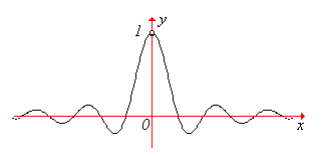
\includegraphics[width=0.7\textwidth]{fig_lim/FunSex_x}
  \caption{Representação da função \mat{\displaystyle f(x)=\frac{\sen x}{x}}}
  \label{fig:lim_Senx/x}
\end{figure}
\nota{
  É possível mostrar também que (\dica experimente!):
    \begin{equation*}
      \displaystyle\lim_{x\to 0}\frac{\cos x-1}{x}=0
  \end{equation*}}
\subsection{Exercícios}
\begin{exer}
  Calcule
  \begin{multicols}{3}
   \begin{compactenum}[a)]
    \item $ \lim_{x\to 0} \frac{\sen 3x}{6x}$\\
  \item $\lim_{x\to 0} \frac{\cos(x)-1}{x}$\\
  \item $\lim_{x\to 0} \frac{\cos(3x)-1}{6x}$
  \end{compactenum}
  \end{multicols}
  \end{exer}
  \begin{resp}
\begin{compactenum}[a)]
\item  $1/2$
\item  $0$
\item $0$
\end{compactenum}
\end{resp}

\section{Limite no infinito}\hypertarget{Lim_no_Inf}{}\label{sec:LimiteNInfinito}
Limites no infinito descrevem a tendência de uma dada função $f(x)$ quando $x\to -\infty$ ou $x\to\infty$.

Dizemos que o limite de $f(x)$ é $L$ quando $x$ tende a $-\infty$, se os valores de $f(x)$ podem ser tomados arbitrariamente próximos de $L$ para valores de $x$ suficientemente pequenos. Neste caso, escrevemos
\begin{equation*}
  \lim_{x\to -\infty} f(x) = L.
\end{equation*}
Veja a Figura \ref{fig:lim_x-infty}.

\begin{figure}[htb]
  \centering
  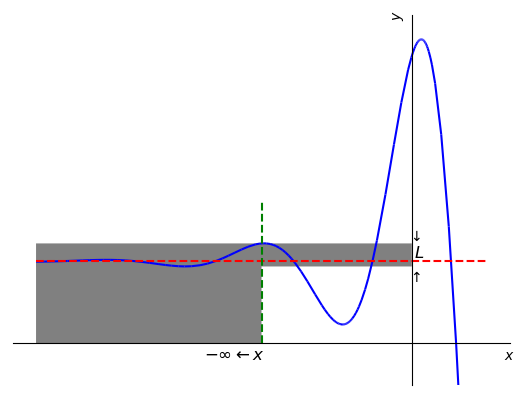
\includegraphics[width=0.7\textwidth]{fig_lim/fig_lim_x-infty}
  \caption{Ilustração da noção de limite de uma função quando $x\to -\infty$.}
  \label{fig:lim_x-infty}
\end{figure}

Analogamente, dizemos que o limite de $f(x)$ é $L$ quando $x$ tende $\infty$, se os valores de $f(x)$ são arbitrariamente próximos de $L$ para valores de $x$ suficientemente grandes. Neste caso, escrevemos
\begin{equation*}
  \lim_{x\to \infty} f(x) = L.
\end{equation*}
Veja a Figura \ref{fig:lim_x2infty}.

\begin{figure}[H]
  \centering
  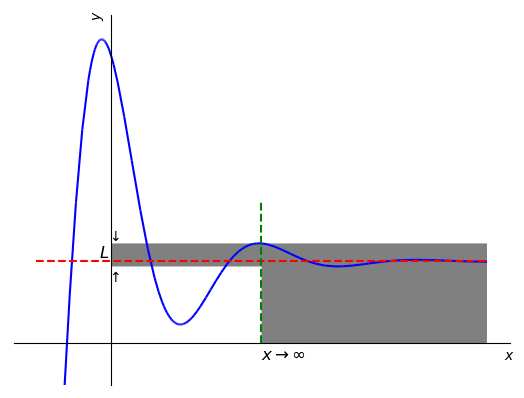
\includegraphics[width=0.55\textwidth]{fig_lim/fig_lim_x2infty}
  \caption{Ilustração da noção de limite de uma função quando $x\to \infty$.}
  \label{fig:lim_x2infty}
\end{figure}
\begin{framed}
\begin{teo}
Seja \(n\in \mathbb{N}\). Então:

\[ \lim\limits_{x \to +\infty}\dfrac{1}{x^n}=0\quad \mbox{e}\quad \lim\limits_{x \to -\infty}\dfrac{1}{x^n}=0. \]
\end{teo}
\end{framed}
\begin{ex}
  Vamos inferir os limites de $f(x) = 1/x$ para $x\to -\infty$ e $x\to \infty$.
  \begin{solution}
  A Figura \ref{fig:lim_xinf_1x} é um esboço do gráfico desta função.

\begin{figure}[H]
  \centering
  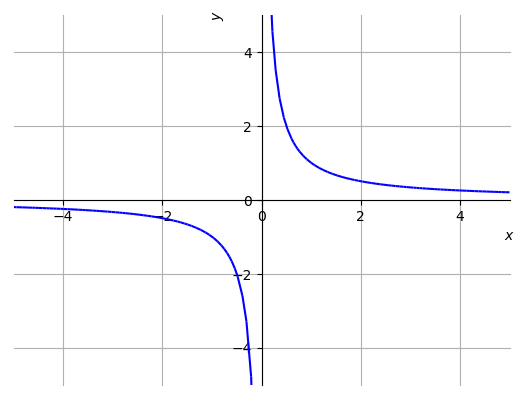
\includegraphics[width=0.6\textwidth]{fig_lim/fig_lim_xinf_1x}
  \caption{Esboço do gráfico de $f(x) = 1/x$.}
  \label{fig:lim_xinf_1x}
\end{figure}

Observamos que quanto menores os valores de $x$, mais próximos de $0$ são os valores de $f(x)=1/x$. Daí, inferimos que
\begin{equation*}
  \lim_{x\to -\infty} \frac{1}{x} = 0
\end{equation*}

Também, quanto maiores os valores de $x$, mais próximos de $0$ são os valores de $f(x)=1/x$. Com isso, podemos concluir que
\begin{equation*}
  \lim_{x\to \infty} \frac{1}{x} = 0
\end{equation*}

Podemos computar estes limites com o \geogebra, usando os seguintes comandos:
\begin{verbatim}
limite(1/x,x,-oo)
limite(1/x,x,oo)
\end{verbatim}
  \end{solution}
\end{ex}

\subsection{Propriedades para o cálculo de limites no infinito}\label{subsec:lim_Propriedades_xinf}
Supondo que $L$, $M$ e $k$ são números reais e
\begin{equation*}
  \lim_{x\to \pm\infty} f(x) = L\quad\text{e}\quad\lim_{x\to\pm\infty}g(x) = M
\end{equation*}
Então, temos as seguintes Propriedades para limites no infinito:
\begin{enumerate}[P1.]
\item Propriedade da soma/diferença
  \begin{equation*}
    \lim_{x\to\pm\infty} (f(x)\pm g(x)) = L\pm M
  \end{equation*}
\item Propriedade do produto
  \begin{equation*}
    \lim_{x\to\pm\infty} f(x)g(x) = LM
  \end{equation*}
\item Propriedade da multiplicação por escalar
  \begin{equation*}
    \lim_{x\to\pm\infty} kf(x) = kL
  \end{equation*}
\item Propriedade do quociente
  \begin{equation*}
    \lim_{x\to\pm\infty} \frac{f(x)}{g(x)} = \frac{L}{M},\quad M\neq 0
  \end{equation*}
\item Propriedade da potenciação
  \begin{equation*}
    \lim_{x\to\pm\infty} (f(x))^k = L^k,\text{ se } L^k\in\mathbb{R}.
  \end{equation*}
\end{enumerate}

\begin{ex}
Calcule $ \lim_{x\to \infty} \pc{\frac{1}{x^2}+1}$\\
\begin{solution}
    \begin{align*}
    \lim_{x\to \infty} \pc{\frac{1}{x^2}+} &= \lim_{x\to \infty} \frac{1}{x^2} + \lim_{x\to \infty}1 \\
                                       &= \left(\lim_{x\to\infty} \frac{1}{x}\right)^2 + 1\\
                                       &= 0^2 + 1 = 1
\end{align*}
\end{solution}
\end{ex}

\begin{ex}\label{ex:liminf_funracio}
  Consideramos o seguinte caso
  \begin{equation*}
    \lim_{x\to \infty} \frac{x^3 - 2x + 1}{2 - 3x^3}
  \end{equation*}
  \begin{solution}
       Observe que não podemos usar a Propriedade do quociente diretamente, pois, por exemplo, não existe o limite do numerador. Para contornar este problema, podemos \textbf{multiplicar e dividir por $\boldsymbol{1/x^3}$ (grau dominante)}, obtendo
  \begin{align*}
    \lim_{x\to\infty} \frac{x^3 - 2x + 1}{2 - 3x^3}\cdot\frac{\frac{1}{x^3}}{\frac{1}{x^3}} = \lim_{x\to\infty} \frac{1-\frac{2}{x^2} + \frac{1}{x^3}}{\frac{2}{x^3}-3}
  \end{align*}
  Então, aplicando a Propriedades do quociente, da soma/subtração e da multiplicação por escalar, temos
  \begin{equation*}
    \lim_{x\to\infty} \frac{x^3 - 2x + 1}{2 - 3x^3} = \lim_{x\to\infty} \frac{1-\frac{2}{x^2} + \frac{1}{x^3}}{\frac{2}{x^3}-3} = -\frac{1}{3}
  \end{equation*}
  \end{solution}
 \end{ex}

\nota{\label{nota:lim_xinf_racio}
  Dados dois polinômios $p(x) = a_nx^n+a_{n-1}x^{n-1}+\cdots + a_0$ e $q(x) = b_mx^m+b_{m-1}x^{m-1}+\cdots + b_0$, temos
  \begin{equation*}
    \lim_{x\to \pm\infty} \frac{p(x)}{q(x)} = \frac{a_nx^n}{b_mx^m}
  \end{equation*}
}

\begin{ex}
  Retornando ao exemplo anterior (Exemplo \ref{ex:liminf_funracio}), temos
  \begin{equation*}
    \lim_{x\to\infty} \frac{x^3 - 2x + 1}{2 - 3x^3} = \lim_{x\to\infty} \frac{x^3}{-3x^3} = -\frac{1}{3}
  \end{equation*}
\end{ex}

\nota{
Quando temos que calcular os limites no infinito de uma função racional na prática, podemos dividir tanto o numerador como o denominador pela maior potência de \(x\) do denominador que aparecer na expressão dada.
}
\subsection{Exercícios Resolvidos}
\begin{exeresol}
  Calculemos os seguintes limites no infinito:\\
  \begin{compactenum}[a)]
  \item \(\lim\limits_{x \to +\infty}\dfrac{7x^2-8x+2}{5x^2+3x-3}\)\\
   \begin{resol}
  Pela observação anterior, dividimos o numerador e o denominador por \(x^2\) (maior potência do denominador) e obtemos:

\[ \lim\limits_{x \to +\infty}\dfrac{7x^2-8x+2}{5x^2+3x-3}= \lim\limits_{x \to +\infty}\dfrac{7-\dfrac{8}{x}+\dfrac{2}{x^2}}{5+\dfrac{3}{x}-\dfrac{3}{x^2}}= \dfrac{\lim\limits_{x \to +\infty} \left(7-\dfrac{8}{x}+\dfrac{2}{x^2} \right)}{\lim\limits_{x \to +\infty}\left(5+\dfrac{3}{x}-\dfrac{3}{x^2}\right)}=\dfrac{7-0+0}{5+0-0}=\dfrac{7}{5}. \]
  \end{resol}
 
  \item \(\lim\limits_{x \to -\infty}\dfrac{12-3x+6x^4}{1+x^6}\)\\
  \begin{resol}
  Nesse caso, dividimos o numerador e o denominador por \(x^6\) e obtemos:
  \begin{align*}
    \lim\limits_{x \to -\infty}\dfrac{12-3x+6x^4}{1+x^6}= \lim\limits_{x \to -\infty}\dfrac{\dfrac{12}{x^6}-\dfrac{3}{x^5}+\dfrac{6}{x^2}}{\dfrac{1}{x^6}+1}\\=\dfrac{\lim\limits_{x \to -\infty} \left( \dfrac{12}{x^6}-\dfrac{3}{x^5}+\dfrac{6}{x^2}\right)}{\lim\limits_{x \to -\infty}\left(\dfrac{1}{x^6}+1 \right)}=\dfrac{0-0+0}{0+1}=0
\end{align*}
  \end{resol}
  \item \(\lim\limits_{x \to +\infty}\dfrac{12x+6}{3-4x}\)\\
  \begin{resol}
  Dividimos o numerador e o denominador por \(x\) e obtemos:

\[ \lim\limits_{x \to +\infty}\dfrac{12x+6}{3-4x}= \lim\limits_{x \to +\infty}\dfrac{12+\dfrac{6}{x}}{\dfrac{3}{x}-4}= \dfrac{\lim\limits_{x \to +\infty} \left( 12+\dfrac{6}{x}\right)}{\lim\limits_{x \to +\infty}\left({\dfrac{3}{x}-4} \right)}=\dfrac{12+0}{0-4}=-3. \]
  \end{resol}
  \end{compactenum}
  \end{exeresol}
  \begin{exeresol}
    Calculemos os seguintes limites no infinito:\\
     \begin{compactenum}[a)]
     \item \(\lim\limits_{x \to -\infty}\sqrt{x^2-2x+4}+x\)\\
  \begin{resol}
  Para que possamos aplicar a metodologia dos exemplos anteriores, precisamos expressar a função como um quociente e, para isso, devemos racionalizar, isto é:

\[ \lim\limits_{x \to -\infty}\sqrt{x^2-2x+4}+x = \lim\limits_{x \to -\infty}\dfrac{\left(\sqrt{x^2-2x+4}+x\right) \left(\sqrt{x^2-2x+4}-x\right)}{\sqrt{x^2-2x+4}-x} \] \[ =\lim\limits_{x \to -\infty}\dfrac{x^2-2x+4-x^2}{\sqrt{x^2-2x+4}-x} =\lim\limits_{x \to -\infty}\dfrac{-2x+4}{\sqrt{x^2-2x+4}-x}. \]
Desde que, \(x\) considera valores negativos que tendem para \(-\infty\), podemos dividir por \(x=-\sqrt{x^2}\), e obteremos:
\[ \lim\limits_{x \to -\infty}\dfrac{-2x+4}{\sqrt{x^2-2x+4}-x}= \lim\limits_{x \to -\infty}\dfrac{-2+\dfrac{4}{x}}{-\sqrt{1-\dfrac{2}{x}+\dfrac{4}{x^2}}-1}=\dfrac{-2+0}{-\sqrt{1-0+0}-1}=1. \]
Portanto, \(\lim\limits_{x \to -\infty}\sqrt{x^2-2x+4}+x=1\).
  \end{resol}
  \item \(\lim\limits_{x \to \infty}\dfrac{\sqrt{x\sqrt{x+\sqrt{x+3}}}}{\sqrt{x+3}}\)\\
  \begin{resol}
  Observamos que \(x\) considera valores positivos, assim, dividimos o numerador e o denominador por \(\sqrt{x}\) e obtemos:
  \begin{align*}
      \lim\limits_{x \to +\infty}\frac{\sqrt{x+\sqrt{x+\sqrt{x+3}}}}{\sqrt{x+3}}&= \lim\limits_{x \to +\infty}\frac{\sqrt{1+\sqrt{\frac{1}{x}+\sqrt{\frac{1}{x^3}+\frac{3}{x^4}}}}}{\sqrt{1+\frac{3}{x}}}\\ &=\frac{\sqrt{1+\sqrt{0+\sqrt{0+0}}}}{\sqrt{1+0}}=1. 
  \end{align*}
  \end{resol}
     \end{compactenum}
  \end{exeresol}
  
  
\subsection{Assíntotas horizontais}\hypertarget{AssintHoriz}{}
A reta $y = L$ é uma assíntota horizontal do gráfico da função $y = f(x)$ se
\begin{equation*}
  \lim_{x\to -\infty} f(x) = L\quad\text{ou}\quad\lim_{x\to\infty} f(x) = L
\end{equation*}

\begin{ex}\label{ex:ass_hor}
  No Exemplo \ref{ex:liminf_funracio}, vimos que
  \begin{equation*}
    \lim_{x\to\infty} \frac{x^3 - 2x + 1}{2 - 3x^3} = -\frac{1}{3}
  \end{equation*}
  Logo, temos que $y=-1/3$ é uma assíntota horizontal do gráfico da função
  \begin{equation*}
    f(x) = \frac{x^3 - 2x + 1}{2 - 3x^3}
  \end{equation*}
  Veja a Figura \ref{fig:ex_ass_horizon}.

      \begin{figure}[htb]
      \centering
      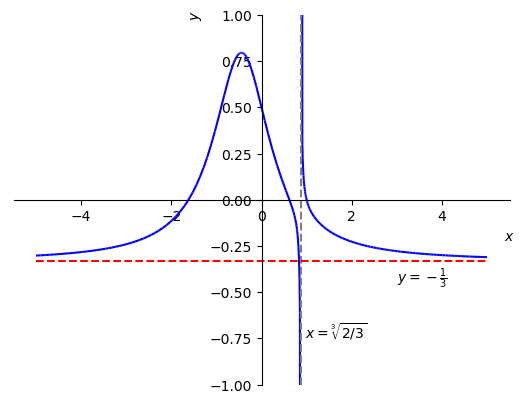
\includegraphics[width=0.7\textwidth]{fig_lim/fig_ex_ass_horizon}
      \caption{Esboço do gráfico da função $\displaystyle f(x) = \frac{x^3 - 2x + 1}{2 - 3x^3}$}
      \label{fig:ex_ass_horizon}
    \end{figure}

  Também, temos
  \begin{equation*}
    \lim_{x\to -\infty} \frac{x^3 - 2x + 1}{2 - 3x^3} = \lim_{x\to\infty} \frac{x^3}{-3x^3} = -\frac{1}{3}
  \end{equation*}
  O que reforça que $y = -1/3$ é uma assíntota horizontal desta função.
\end{ex}

\begin{ex}\normalfont{(Função exponencial natural)}\label{ex:lim_exp_x-inf}
  \begin{equation*}
    \lim_{x\to -\infty} e^x = 0,
  \end{equation*}
  donde temos que $y=0$ é uma assíntota horizontal da função exponencial natural. Veja a Figura \ref{fig:lim_ex_xinf_exp}.

  \begin{figure}[H]
    \centering
    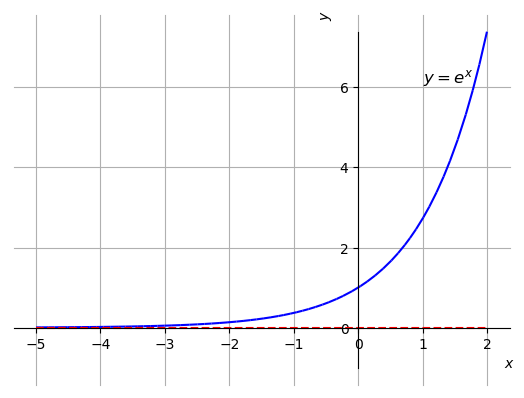
\includegraphics[width=0.7\textwidth]{fig_lim/fig_ex_xinf_exp}
    \caption{Esboço do gráfico de $f(x)=e^x$.}
    \label{fig:lim_ex_xinf_exp}
  \end{figure}
\end{ex}

\begin{ex}\normalfont{(Função logística)}
  Na ecologia, a \href{https://pt.wikipedia.org/wiki/Fun\%C3\%A7\%C3\%A3o_log\%C3\%ADstica}{função logística}
    \begin{equation*}
      P(t) = \frac{K}{1 + \left(\frac{K-P_0}{P_0}e^{-rt}\right)}
    \end{equation*}
    é um modelo de crescimento populacional de espécies, sendo $P(t)$ o número de indivíduos da população no tempo $t$. O parâmetro $P_0$ é o número de indivíduos na população no tempo inicial $t=0$, $r>0$ é a proporção de novos indivíduos na população devido a reprodução e $K$ é o limite de saturação do crescimento populacional (devido aos recursos escassos como alimentos, território e tratamento a doenças). Observamos que
    \renewcommand{\CancelColor}{\color{red}}%mudando a cor do traço de cancelamento
    \begin{equation*}
      \lim_{t\to\infty} P(t) = \lim_{t\to\infty} \frac{K}{1 + \left(\frac{K-P_0}{P_0}\cancelto{0}{e^{-rt}}\right)} = K
    \end{equation*}
    Ou seja, $P(t) = K$ é uma assíntota horizontal ao gráfico de $P = P(t)$ e é o limite de saturação do crescimento populacional. Na Figura \ref{fig:liminf_ex_funlogic}, temos o esboço do gráfico da função logística para $t\geq 0$.

    \begin{figure}[H]
      \centering
      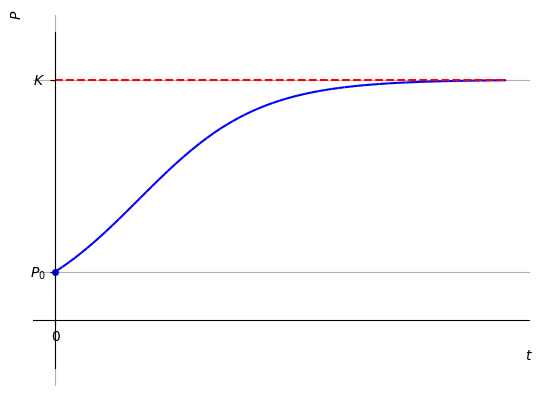
\includegraphics[width=0.7\textwidth]{fig_lim/fig_liminf_ex_funlogic}
      \caption{Esboço do gráfico da função logística.}
      \label{fig:liminf_ex_funlogic}
    \end{figure}
\end{ex}

\subsection{Exercícios resolvidos}

\begin{exeresol}
  Calcule
  \begin{equation*}
    \lim_{x\to \infty} \frac{1}{x-1}+1
  \end{equation*}
  \begin{resol}
  Utilizando a Propriedade da soma para limites no infinito, temos
  \begin{align*}
    \lim_{x\to\infty} \frac{1}{x-1} + 1 &= \lim_{x\to \infty} \frac{1}{x-1} + \lim_{x\to 1} 1\\
                                        &= \lim_{x\to \infty} \left(\frac{1}{x-1}\right)+1
  \end{align*}
  observando que $\lim_{x\to \infty}1/(x-1)$ existe. De fato, o gráfico de $g(x) = 1/(x-1)$ é uma translação de uma unidade à esquerda da função $f(x)=1/x$. Uma translação horizontal finita não altera o comportamento da função para $x\to \infty$. Portanto, como $f(x)=1/x\to\infty$ quando $x\to\infty$, temos que $g(x)=f(x-1)=1/(x-1)\to\infty$ quando $x\to\infty$, i.e.
  \begin{equation*}
    \lim_{x\to\infty}\frac{1}{x-1} = 0
  \end{equation*}
  Portanto, concluímos que
  \begin{equation*}
    \lim_{x\to \infty} \frac{1}{x-1} + 1 = 1
  \end{equation*}

  
  Com o \geogebra, podemos computar este limite com o seguinte comando:
\begin{verbatim}
limit(1/(x-1)+1,x,oo)
\end{verbatim}
 
\end{resol}
\end{exeresol}

\begin{exeresol}
  Determine a(s) assíntota(s) horizontal(ais) do gráfico da função
  \begin{equation*}
    f(x) = \frac{3 - x + 4x^4 - 10x^3}{x^2 + 2x^4 -x}
  \end{equation*}
\end{exeresol}
\begin{resol}
  Uma reta $y = L$ é assíntota horizontal do gráfico de $f$, quando
  \begin{equation*}
    \lim_{x\to\pm\infty} f(x) = L
  \end{equation*}
  Começamos com $x\to-\infty$, temos
  \begin{align*}
    \lim_{x\to-\infty} f(x) &= \lim_{x\to-\infty} \frac{3 - x + 4x^4 - 10x^3}{x^2 + 2x^4 -x} \\
                            &= \lim_{x\to -\infty} \frac{4x^4}{2x^4} = 2
  \end{align*}
  Logo, $y=2$ é assíntota horizontal ao gráfico de $f(x)$.

  Agora, vamos ver a tendência da função para $x\to\infty$, temos
  \begin{equation*}
    \lim_{x\to\infty} f(x) = \lim_{x\to\infty} \frac{3 - x + 4x^4 - 10x^3}{x^2 + 2x^4 -x} = \frac{4}{2} = 2
  \end{equation*}
  Portanto, concluímos que $y=2$ é a única assíntota horizontal ao gráfico da função $f$.
\end{resol}

\begin{exeresol}
  Calcule
  \begin{equation*}
    \lim_{x\to\infty} \frac{\sqrt{1+x^2}}{2x}
  \end{equation*}
\end{exeresol}
\begin{resol}
  Seguindo a ideia aplicada no Exemplo \ref{ex:liminf_funracio}, temos
  \begin{align*}
    \lim_{x\to\infty} \frac{\sqrt{1+x^2}}{2x} &= \lim_{x\to\infty} \frac{\sqrt{1+x^2}}{x}\cdot \frac{\frac{1}{\sqrt{x^2}}}{\frac{1}{\sqrt{x^2}}} \\
                                             &= \lim_{x\to\infty} \frac{\sqrt{\frac{1}{x^2}+\frac{x^2}{x^2}}}{2\frac{x}{\sqrt{x^2}}}
  \end{align*}
  Lembramos que $\sqrt{x^2}=|x|$. Como $x\to\infty$, temos $\sqrt{x^2} = |x|=x$. Logo,
  \begin{align*}
    \lim_{x\to\infty} \frac{\sqrt{\frac{1}{x^2}+\frac{x^2}{x^2}}}{2\frac{x}{\sqrt{x^2}}} &= \lim_{x\to\infty} \frac{\sqrt{\frac{1}{x^2}+\frac{x^2}{x^2}}}{2\frac{x}{|x|}}\\
                                                                                         &= \lim_{x\to\infty} \frac{\sqrt{\frac{1}{x^2}+1}}{2\frac{x}{x}}\\
                                                                                         &= \lim_{x\to\infty} \frac{1}{2}\sqrt{\frac{1}{x^2}+1}\\
                                                                                         &= \frac{1}{2}\sqrt{\lim_{x\to\infty} \frac{1}{x^2}+1}\\
                                                                                         &= \frac{1}{2}
  \end{align*}
\end{resol}

\begin{exeresol}
  Calcule
  \begin{equation*}
    \lim_{x\to \infty} e^{-x}
  \end{equation*}
\end{exeresol}
\begin{resol}
  Observamos que o gráfico de $f(x)=e^{-x}$ é uma reflexão em torno do eixo $y$ do gráfico da função $g(x)=e^x$. No Exemplo \ref{ex:lim_exp_x-inf}, vimos que
  \begin{equation*}
    \lim_{x\to -\infty} g(x) = \lim_{x\to -\infty} e^{x} = 0,
  \end{equation*}
  logo
  \begin{equation*}
    \lim_{x\to \infty} e^{-x} = \lim_{x\to \infty} g(-x) = \lim_{x\to -\infty} g(x) = 0.
  \end{equation*}
  Veja o esboço do gráfico de $f(x)=e^{-x}$ na Figura \ref{fig:exeresol_lim_exp_xinf}.

  \begin{figure}[htb]
    \centering
    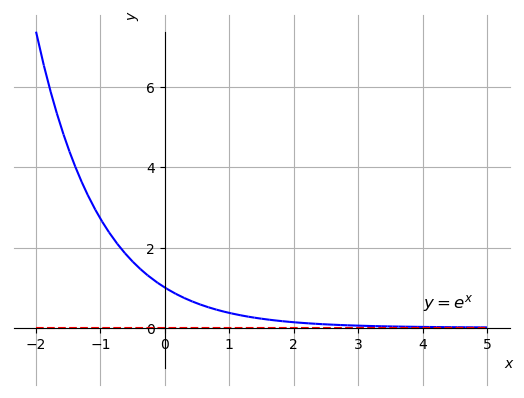
\includegraphics[width=0.7\textwidth]{fig_lim/fig_exeresol_lim_exp_xinf}
    \caption{Esboço do gráfico de $f(x)=e^{-x}$.}
    \label{fig:exeresol_lim_exp_xinf}
  \end{figure}  

  
  Com o \geogebra, podemos computar este limite com o seguinte comando:
\begin{verbatim}
limit(exp(-x),x,oo)
\end{verbatim}
 
\end{resol}

\subsection{Exercícios}
\begin{exer}
  Calcule
  \begin{multicols}{2}
  \begin{enumerate}[a)]
\item $\displaystyle \lim_{x\to -\infty} e^x+1$
\item $\displaystyle \lim_{x\to \infty} 3 + e^{-x}$
\item $\displaystyle \lim_{x\to \infty} 2e^{-x}-1$
\item $\displaystyle \lim_{x\to -\infty} e-e^{x}$
\end{enumerate}
  \end{multicols}
\end{exer}
\begin{resp}
  a)~$1$; b)~$3$; c)~$-1$; d)~$e$
\end{resp}

\begin{exer}
    \begin{equation*}
    \lim_{x\to -\infty} \frac{\sqrt{1+x^2}}{2x}
  \end{equation*}
\end{exer}


\begin{resp}
  $-1/2$
\end{resp}

\begin{exer}
  Calcule
  \begin{equation*}
    \lim_{x\to -\infty} \cos x
  \end{equation*}
\end{exer}
\begin{resp}
  não existe.
\end{resp}

\begin{exer}
  Calcule:
  \begin{enumerate}[a)]
  \item $\displaystyle\lim_{x\to \infty} \sqrt{1+e^{-x}}$.
  \item $\displaystyle\lim_{x\to -\infty} \frac{1-2x}{x+3} -e^{x} - 1$
  \end{enumerate}
\end{exer}
\begin{resp}
  a)~$1$; b)~$-3$
\end{resp}
\newpage
\section{Limites infinitos}\hypertarget{LimInf}{}\label{sec:limites_inf}

\figtext{0.1cm}{r}{0.4}{
 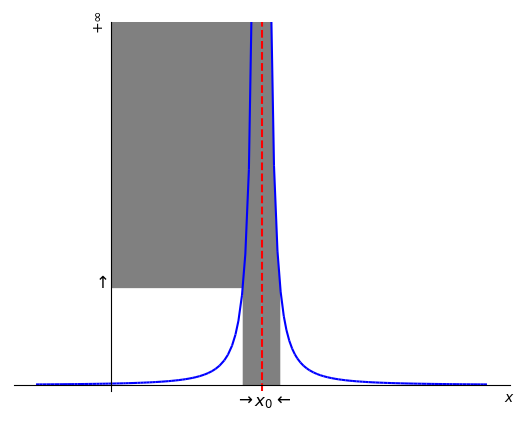
\includegraphics[width=1\textwidth]{fig_lim/fig_liminf}
 \vspace{-0.9cm}
   \captionof{figure}{\hspace{-0.1cm}\footnotesize{$f(x)\to\infty$ quando $x\to x_0$.}}
   \label{fig:liminf2}
    }
\noindent O limite de uma função nem sempre existe. Entretanto, em muitos destes casos, podemos concluir mais sobre a tendência da função. Por exemplo, dizemos que o limite de uma dada função $f(x)$ é infinito quando $x$ tende a um número $x_0$ e $f(x)$ torna-se arbitrariamente grande para todos os valores de $x$ suficientemente próximos de $x_0$, mas $x\neq 0$. Neste caso, escrevemos
\begin{equation*}
  \lim_{x\to x_0} f(x) = \infty
\end{equation*}
A Figura \ref{fig:liminf2}, é uma ilustração de $f(x)\to\infty$ quando $x\to x_0$

Analogamente, dizemos que o limite de uma dada função $f(x)$ é menos infinito quando $x$ tende a $x_0$, e $f(x)$ torna-se arbitrariamente pequeno para valores de $x$ suficientemente próximos de $x_0$, com $x\neq x_0$. Neste caso, escrevemos

\begin{equation*}
  \lim_{x\to x_0} f(x) = -\infty
\end{equation*}
\begin{comment}
\begin{figure}[htb]
  \centering
  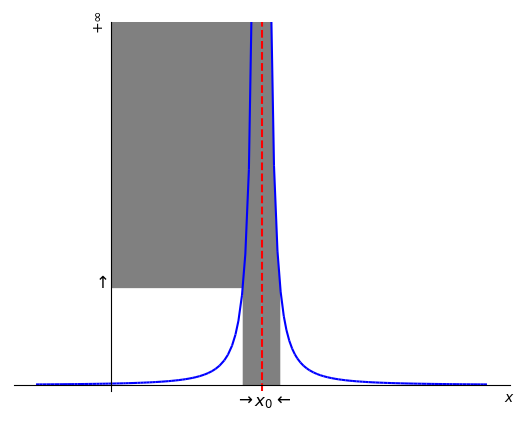
\includegraphics[width=0.7\textwidth]{fig_lim/fig_liminf}
  \caption{Ilustração de $f(x)\to\infty$ quando $x\to x_0$.}
  \label{fig:liminf}
\end{figure}
\end{comment}

\begin{ex}
  Vejamos o caso de
  \begin{equation*}
    \lim_{x\to 0} \frac{1}{x^2}
  \end{equation*}
  Ao tomarmos $x$ próximo de $x_0=0$, obtemos os seguintes valores de $f(x)$:
  \begin{center}
    \begin{tabular}[H]{l|ccc|c|ccc}
      x & $-10^{-1}$ & $-10^{-2}$ & $-10^{-3}$ & $\rightarrow 0 \leftarrow$ & $10^{-3}$ & $10^{-2}$ & $10^{-1}$ \\\hline
      f(x) & $-10^{2}$ & $-10^{4}$ & $-10^{6}$ & $\rightarrow \infty \leftarrow$ & $10^{6}$ & $10^{4}$ & $10^{2}$
    \end{tabular}
  \end{center}
  Veja o esboço do gráfico de $f(x)$ na Figura \ref{fig:ex_liminf_1x2}.

\begin{figure}[H]
  \centering
  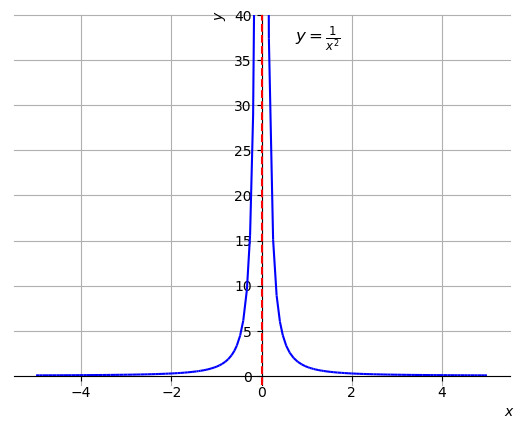
\includegraphics[width=0.63\textwidth]{fig_lim/fig_ex_liminf_1x2}
  \caption{Esboço do gráfico de $f(x)=1/x^2$.}
  \label{fig:ex_liminf_1x2}
\end{figure}  

  Podemos concluir que os valores de $f(x)$ podem ser tomados arbitrariamente grandes ao escolhermos qualquer $x$ suficientemente próximo de $0$, com $x\neq 0$. I.e.,
  \begin{equation*}
    \lim_{x\to 0}\frac{1}{x^2} = \infty
  \end{equation*}

 No \geogebra, podemos computar este limite com o seguinte comando:
\begin{verbatim}
limit(1/x**2,x,0)
\end{verbatim}
  
\end{ex}

\begin{framed}
\begin{definition}
Definimos os limites laterais infinitos
\begin{equation*}
  \lim_{x\to x_0^-} f(x) = \infty\quad\text{e}\quad\lim_{x\to x_0^+} f(x) = \infty
\end{equation*}
No primeiro caso, os valores de $f(x)$ são arbitrariamente grandes conforme os valores de $x\to x_0$ e $x<x_0$. No segundo caso, os valores de $f(x)$ são arbitrariamente grandes conforme os valores de $x\to x_0$ e $x>x_0$.

De forma similar, definimos os limites laterais $f(x)\to -\infty$ quando $x\to x_0^{\pm}$.
\end{definition}
\end{framed}

\nota{
\begin{compactenum}[a.]
\item  Desde que os símbolos \(+\infty\) e \(-\infty\) não são números reais, nenhum dos limites infinitos existem de fato.
\item O termo o limite existe será usado somente quando o limite é um número real.
\end{compactenum}
}
\begin{framed}
\begin{teo}\label{teo:LimInf}
Seja \(n\in \mathbb{N}\). Então:

\[ \lim\limits_{x \to 0^{+}}\dfrac{1}{x^n}=+\infty \quad \mbox{e}\quad \lim\limits_{x \to 0^{-}}\dfrac{1}{x^n}= \left\{ \begin{array}{ccl} -\infty,& & \mbox{ se }\,\, n\,\, \mbox{é ímpar};\\ +\infty,& & \mbox{ se }\,\, n\,\, \mbox{é par}. \end{array}\right. \]
\end{teo}
\end{framed}

\begin{ex}
  Alguns casos particulares do Teorema \ref{teo:LimInf} são:

\[ \lim\limits_{x \to 0^{+}}\dfrac{1}{x^5}=+\infty, \quad\lim\limits_{x \to 0^{+}}\dfrac{1}{x^4}=+\infty, \quad \lim\limits_{x \to 0^{-}}\dfrac{1}{x^3}=-\infty, \quad \lim\limits_{x \to 0^{+}}\dfrac{1}{x^6}=+\infty. \]
O seguinte resultado apresenta algumas propriedades que nos permitem calcular limites infinitos.
\end{ex}

\begin{ex}
  Observe que
  \begin{equation*}
    \nexists \lim_{x\to 0} \frac{1}{x}
  \end{equation*}
  e que não podemos concluir que este limite é $\infty$ ou $-\infty$. Isto ocorre, pois
  \begin{equation*}
    \lim_{x\to 0^-} \frac{1}{x} = -\infty\quad\text{e}\quad\lim_{x\to 0^+} \frac{1}{x} = +\infty
  \end{equation*}
\end{ex}

\begin{ex}
  \begin{equation*}
    \lim_{x\to 1^+} \frac{1}{x-1} = \infty
  \end{equation*}
  De fato, conforme tomamos valores de $x$ próximos de $1$, com $x>1$, os valores de $f(x) = 1/(x-1)$ tornam-se cada vez maiores. Veja o esboço do gráfico de $f(x)$ na Figura \ref{fig:ex_liminf_1x}.

\begin{figure}[H]
  \centering
  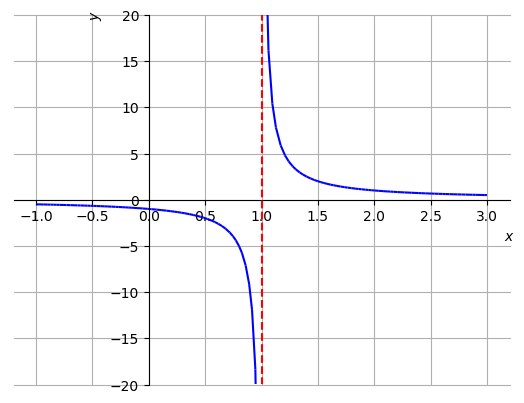
\includegraphics[width=0.7\textwidth]{fig_lim/fig_ex_liminf_1x}
  \caption{Esboço do gráfico de $f(x)=1/(x-1)$.}
  \label{fig:ex_liminf_1x}
\end{figure}  
\end{ex}

\begin{ex}
  \begin{equation*}
    \lim_{x\to -1} \frac{-1}{(x+1)^2} = -\infty
  \end{equation*}
  De fato, podemos inferir este limite a partir do gráfico da função $f(x) = -1/(x+1)^2$. Este é uma translação de uma unidade à esquerda do gráfico de $y = 1/x^2$, seguida de uma reflexão em torno de eixo $x$. Veja a Figura \ref{fig:ex_liminf-1x2}.

  \begin{figure}[H]
    \centering
    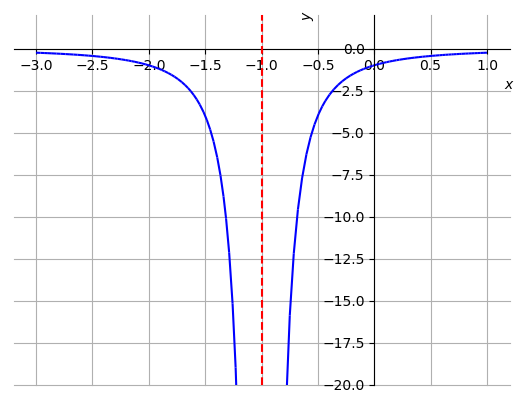
\includegraphics[width=0.6\textwidth]{fig_lim/fig_ex_liminf-1x2}
    \caption{Esboço do gráfico de $f(x)=-1/(x+1)^2$}
    \label{fig:ex_liminf-1x2}
  \end{figure}
\end{ex}

\subsection{Regra (generalização)}
Se no cálculo de um limite ocorrer uma situação do tipo $\frac{k}{0}, k\neq 0$, então:
$$\left\{\begin{array}{ccc}
     \frac{k}{0^+}=\infty, k>0&  \textrm{ e }&\frac{k}{0^+}=-\infty, k<0\\
   \frac{k}{0^-}=-\infty, k>0&  \textrm{ e }&\frac{k}{0^-}=\infty, k<0
\end{array}\right.$$

Desta Tabela podemos perceber que $\frac{k}{\pm\infty}=0$. Se o denominador tende ao infinito com o
numerador constante, a razão se aproxima de zero, conforme vimos na seção \ref{sec:LimiteNInfinito}.

\subsection{Assíntotas verticais}\hypertarget{AssintVert}{}
Uma reta $x=x_0$ é uma {\bf assíntota vertical} do gráfico de uma função $y = f(x)$ se
\begin{equation*}
  \lim_{x\to x_0^-} f(x) = \pm\infty\quad\text{ou}\quad\lim_{x\to x_0^+} f(x) = \pm\infty
\end{equation*}

\begin{ex}
  O gráfico da função $f(x)=-1/|x|$ tem uma assíntota vertical em $x=0$, pois $\lim_{x\to 0} \frac{-1}{|x|} = -\infty$.
  \begin{comment}
   \begin{equation*}
    \lim_{x\to 0} \frac{-1}{|x|} = -\infty
  \end{equation*}
  \end{comment}
   Veja o esboço de seu gráfico na Figura \ref{fig:ex_lim_assvert_1}.

  \begin{figure}[H]
    \centering
    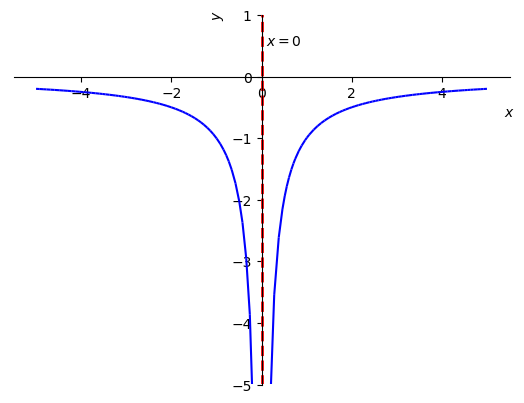
\includegraphics[width=0.65\textwidth]{fig_lim/fig_ex_lim_assvert_1}
    \caption{Esboço do gráfico de $f(x)=-1/|x|$.}
    \label{fig:ex_lim_assvert_1}
  \end{figure}  
\end{ex}
\renewcommand{\CancelColor}{\color{red}}%mud

\begin{ex}
  A função $\displaystyle f(x) = \frac{x^3 + 2x^2 - 4x - 8}{x^2 - 1}$ não está definida para valores de $x$ tais que seu denominador se anule, i.e.
    \begin{equation*}
      x^2 - 1 = 0 \Rightarrow x_0=-1\quad\text{ou}\quad x_1=1.
    \end{equation*}
    Nestes pontos o gráfico de $f$ pode ter assíntotas verticais. De fato, temos
    \begin{align*}
      \lim_{x\to -1^+} \frac{\cancelto{-3}{x^3 + 2x^2 - 4x - 8}}{\cancelto{0^-}{x^2-1}} &=  +\infty\quad & \textrm{e}\qquad &
      \lim_{x\to -1^-} \frac{\cancelto{-3}{x^3 + 2x^2 - 4x - 8}}{\cancelto{0^+}{x^2-1}} &=  -\infty
    \end{align*}
    e, também, temos
    \begin{align*}
      \lim_{x\to 1^+} \frac{\cancelto{-9}{x^3 + 2x^2 - 4x - 8}}{\cancelto{0^+}{x^2-1}} &= -\infty\\      
      \lim_{x\to 1^-} \frac{\cancelto{-9}{x^3 + 2x^2 - 4x - 8}}{\cancelto{0^-}{x^2-1}} &= +\infty
    \end{align*}
    Com isso, temos que as retas $x=-1$ e $x=1$ são assíntotas verticais ao gráfico da função $f$. Veja a Figura \ref{fig:ex_lim_assvert_racio} para o esboço do gráfico desta função.
    \begin{figure}[H]
      \centering
      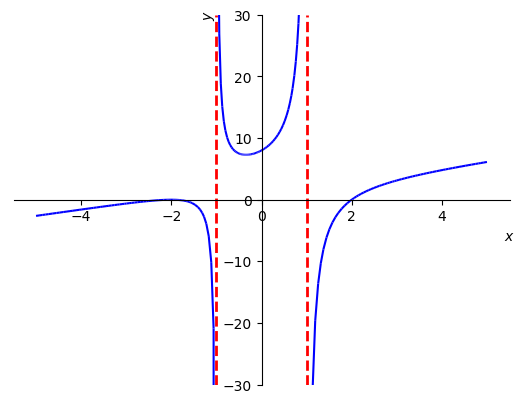
\includegraphics[width=0.65\textwidth]{fig_lim/fig_ex_lim_assvert_racio}
      \caption{Esboço do gráfico da função $\displaystyle f(x) = \frac{x^3 + 2x^2 - 4x - 8}{x^2 - 1}$.}
      \label{fig:ex_lim_assvert_racio}
    \end{figure}
\end{ex}

\begin{ex}\normalfont{(Função logarítmica)}
  A função logarítmica natural $y = \ln x$ é tal que
  \begin{equation*}
    \lim_{x\to 0^+} \ln x = -\infty
  \end{equation*}
  i.e., $x=0$ é uma assíntota vertical ao gráfico de $\ln x$. Isto decorre do fato de $y = \ln x$ ser a função inversa de $y = e^x$ e, esta, ter uma assíntota horizontal $y=0$\footnote{Veja o Exemplo \ref{ex:lim_exp_x-inf}.}. A Figura \ref{fig:ex_lim_assvert_lnx} é um esboço do gráfico da função  $\ln x$.

    \begin{figure}[H]
      \centering
      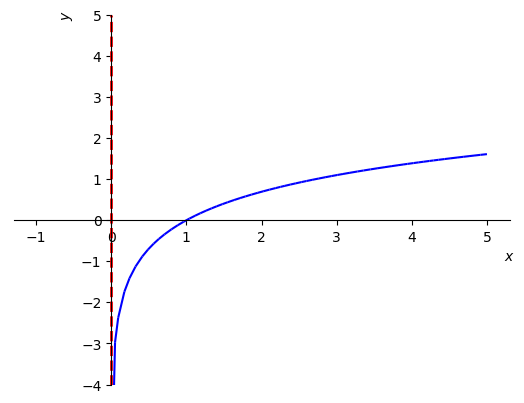
\includegraphics[width=0.6\textwidth]{fig_lim/fig_ex_lim_assvert_lnx}
      \caption{Esboço do gráfico da função logaritmo natural.}
      \label{fig:ex_lim_assvert_lnx}
    \end{figure}  
\end{ex}

\begin{ex}
  As funções trigonométricas $y = \sec x$ e $\displaystyle y = \tg x$ têm assíntotas verticais $x = (2k+1)\frac{\pi}{2}$ para $k$ inteiro. Veja as Figuras \ref{fig:co_tg_graficos}.
\end{ex}

\begin{ex}
  As funções trigonométricas $y = \cosec x$ e $\displaystyle y = \cotg x$ têm assíntotas verticais $x = k\pi$ para $k$ inteiro. Veja as Figuras \ref{fig:co_sec_graficos}.
\end{ex}

\subsection{Exercícios resolvidos}
\begin{exeresol}
  Calcule os limites:\\
  \begin{compactenum}[a)]
  \item \(\lim\limits_{x \to 2^{+}} \dfrac{x+2}{x^2-4}\)\\
    \begin{resol}
  \(\lim\limits_{x \to 2^{}} \dfrac{x+2}{x^2-4}=\lim\limits_{x \to 2^{}} \dfrac{\cancel{x+2}}{(x-2)\cancel{(x+2)}}=\lim\limits_{x \to 2^{}} \dfrac{1}{x-2}=\infty\).
\end{resol}
\item  \(\lim\limits_{x \to 4^{-}} \dfrac{\sqrt{16-x^2}}{x-4}\)\\
  \begin{resol}
    \[ \begin{array}{rcl} \lim\limits_{x \to 4^{-}} \dfrac{\sqrt{16-x^2}}{x-4} & = & \lim\limits_{x \to 4^{-}} \dfrac{16-x^2}{(x-4)\sqrt{16-x^2}} = \lim\limits_{x \to 4^{-}} \dfrac{(4-x)(4+x)}{(x-4)\sqrt{16-x^2}}\\ &=& -\lim\limits_{x \to 4^{-}} \dfrac{4+x}{\sqrt{16-x^2}} =-\dfrac{8}{0^{+}}=-\infty. \end{array} \]
  \end{resol}
  \item \(\lim\limits_{x \to 4^{-}} \dfrac{\left\lfloor x\right\rfloor-4}{x-4}\)\\
  \begin{resol}
  Desde que \(x \to 4^{-}\), temos \(x\in [3,4)\Rightarrow \left\lfloor x\right\rfloor =3\), logo,

\[ \lim\limits_{x \to 4^{-}} \dfrac{\left\lfloor x\right\rfloor-4}{x-4}= \lim\limits_{x \to 4^{-}} \dfrac{3-4}{x-4} =\lim\limits_{x \to 4^{-}} \dfrac{-1}{x-4} = -\dfrac{1}{0^{-}}=+\infty. \]
  \end{resol}
  \end{compactenum}
\end{exeresol}
\subsection{Limites infinitos no infinito}
Da mesma forma que os limites em números reais, os limites no infinito podem deixar de existir, por exemplo, quando valores de \(f(x)\) crescerem ou decrescerem ilimitadamente quando \({x \to +\infty}\) ou \({x \to -\infty}\). 

Escrevemos
\begin{equation*}
  \lim_{x\to\infty} f(x)=\infty,
\end{equation*}
quando os valores da função $f$ são arbitrariamente grandes para todos os valores de $x$ suficientemente grandes. De forma análoga, definimos
\begin{equation*}
  \lim_{x\to -\infty} f(x)=\infty,\quad\lim_{x\to \infty} f(x)=-\infty\quad\text{e}\quad\lim_{x\to -\infty} f(x)=-\infty.
\end{equation*}

A Tabela abaixo apresenta situações de soma e produto de infinitos que usaremos com frequência.
\begin{framed}
$\left\{\begin{array}{l}
   (\pm\infty)\cdot (\pm\infty)=+\infty\\
    (\mp\infty)\cdot (\pm\infty)=-\infty   \\
     (\pm\infty)+ (\pm\infty)=+\infty\\
      (\pm\infty)- (\pm\infty)=? \textrm{(ideterminação!)}
\end{array}\right.$\hfill
$\left\{\begin{array}{l}
   (\pm\infty)\cdot k=\pm\infty, \textrm{ se } k>0\\
   (\pm\infty)\cdot k=\mp\infty, \textrm{ se } k<0\\
    (\pm\infty)+ k=\pm\infty\\
      (\pm\infty)- k=\pm\infty\\
\end{array}\right.$
\end{framed}
Vale ressaltar ainda que, se $n$ é um \textbf{natural não nulo}, então:\\
$\displaystyle\lim_{\to +\infty} x^n=+\infty\quad$ e $\quad\displaystyle\lim_{\to -\infty} x^n=\left\{\begin{array}{l}
  +\infty, n \textrm{ par}\\
     -\infty, n \textrm{ impar}
\end{array}\right.$

\begin{ex}
  Vejamos os seguintes casos:
  \begin{multicols}{2}
 \begin{enumerate}[a)]
  \item $\displaystyle\lim_{x\to\infty} x^2 = \infty$
  \item $\displaystyle\lim_{x\to -\infty} x^2 = \infty$
  \item $\displaystyle\lim_{x\to -\infty} x^3 = -\infty$
  \item $\displaystyle\lim_{x\to \infty} e^x = \infty$
  \item $\displaystyle\lim_{x\to \infty} \ln x = \infty$
  \item $\displaystyle\lim_{x\to -\infty} e^{-x} = \infty$
  \end{enumerate}
  \end{multicols}
  \end{ex}
  
\begin{ex}\label{ex:liminf_poli}
  \begin{align*}
    \lim_{x\to \infty} x^3 - 10x^2 + 300 &= \lim_{x\to \infty} \frac{x^3 - 10x^2 + 300}{1}\cdot\frac{\frac{1}{x^3}}{\frac{1}{x^3}}\\
                                         &= \lim_{x\to \infty} \frac{1 - \cancelto{0^+}{\frac{10}{x}} + \cancelto{0^+}{\frac{300}{x^3}}}{\cancelto{0^+}{\frac{1}{x^3}}} = \infty                                
  \end{align*}
\end{ex}

\begin{ex}
  Retornando ao exemplo anterior, temos
  \begin{align*}
    \lim_{x\to \infty} x^3 - 10x^2 + 300 &= \lim_{x\to \infty} x^3 = \infty
  \end{align*}
\end{ex}

\subsection{Exercícios resolvidos}

\begin{exeresol}
  Calcule\\
  \begin{compactenum}[a)]
  \item \mat{\lim_{x\to 1^-} \frac{x-2}{1-x}}\\
  \begin{resol}
  Temos
  \begin{align*}
    \lim_{x\to 1^-} \frac{\cancelto{-1}{x-2}}{\cancelto{0^+}{1-x}} = -\infty
  \end{align*}

  Outra forma de calcular este limite é observar que $y = 1-x\to 0^+$ quando $x\to 1^-$. Assim, fazendo a mudança de variável $y = x-1$, temos
  \begin{equation*}
    \lim_{x\to 1^-} \frac{x-2}{1-x} = \lim_{y\to 0^+} \frac{y+1-2}{y} = \lim_{y\to 0^+} \frac{y-1}{y} = -\infty
  \end{equation*}
 \end{resol}
 \item  \mat{\lim_{x\to 1} \ln |x-1|}\\
 \begin{resol}
  Começamos observando que
  \begin{equation*}
    \ln |x-1| = \left\{
      \begin{array}{ll}
        \ln(1-x), & x < 1\\
        \ln(x-1), &x > 1
      \end{array}
    \right.
  \end{equation*}
  Então, calculando o limite lateral à esquerda, temos
  \begin{align*}
    \lim_{x\to 1^-} \ln |x-1| &= \lim_{x\to 1^-} \ln(1-x)\\
                              &= \lim_{y\to 0^+} \ln y = -\infty\footnote{Observe que $1-x\to 0^+$ quando $x\to 1^-$}
  \end{align*}
  Por outro lado, temos
  \begin{align*}
    \lim_{x\to 1^+} \ln |x-1| &= \lim_{x\to 1^+} \ln(x-1)\\
                              &= \lim_{y\to 0^+} \ln y = -\infty\footnote{Observe que $x-1\to 0^+$ quando $x\to 1^+$}
  \end{align*}
  Portanto, concluímos que
  \begin{equation*}
    \lim_{x\to 1} \ln |x-1| = -\infty.
  \end{equation*}
  \end{resol}
\item $ \lim_{x\to \infty} \frac{x^3+2x^2-4x-8}{x^2-1}$\\
\begin{resol}
  Tratando-se de uma função racional, temos\footnote{Veja a Observação \ref{nota:lim_xinf_racio}. Veja, também, o gráfico desta função na Figura \ref{fig:ex_lim_assvert_racio}.}
  \begin{equation*}
    \lim_{x\to \infty} \frac{x^3+2x^2-4x-8}{x^2-1} = \lim_{x\to\infty} \frac{x^3}{x^2} = \lim_{x\to \infty} x = \infty
  \end{equation*}
\end{resol}
\item  \mat{\lim_{x\to \infty} e^{1-x^2}}\\
\begin{resol}
   Observamos que $1-x^2\to -\infty$ quando $x\to \infty$. Desta forma, fazendo a mudança de variáveis $y = 1 - x^2$, temos
  \begin{equation*}
    \lim_{x\to\infty} e^{1-x^2} = \lim_{y\to -\infty} e^y = 0
  \end{equation*}
\end{resol}
  \end{compactenum}
 \end{exeresol}
\begin{exeresol}
  Calculemos os seguintes limites:
  \begin{compactenum}[a)]
  \item \(\lim\limits_{x \to +\infty} (-8x^{12}+5x^7-5x^3+2x-67)\)\\
  \begin{resol}
    \(\lim\limits_{x \to +\infty} (-8x^{12}+5x^7-5x^3+2x-67)=\lim\limits_{x \to +\infty} (-8x^{12})=-\infty\).
  \end{resol}
  \item \(\lim\limits_{x \to -\infty} \dfrac{7x^{9}-456x^5-6700}{1000x^3-1}\)\\
  \begin{resol}
    \(\lim\limits_{x \to -\infty} \dfrac{7x^{9}-456x^5-6700}{1000x^3-1}=\lim\limits_{x \to -\infty} \dfrac{7x^{9}}{1000x^3}=\lim\limits_{x \to -\infty} \dfrac{7x^{6}}{1000}=+\infty\).
  \end{resol}
\item \(\lim\limits_{x \to +\infty} \dfrac{\sqrt{x^2+9}}{x+4}\)\\ 
  \begin{resol}
    O limite é da forma \(\infty/\infty\). Dividimos o numerador e o denominador por \(x=\sqrt{x^2},\,x>0\) , obtemos \[\lim\limits_{x \to \infty} \dfrac{\sqrt{x^2+9}}{x+4}= \lim\limits_{x \to +\infty} \dfrac{\dfrac{\sqrt{x^2+9}}{\sqrt{x^2}}}{\dfrac{x+4}{x}} = \lim\limits_{x \to +\infty} \dfrac{\sqrt{1\dfrac{9}{x^2}}}{1+\dfrac{4}{x}}=1\].
  \end{resol}
  \item \(\lim\limits_{x \to -\infty} \dfrac{\sqrt{x^2+9}}{x+4}\)\\
  \begin{resol}
    Esse limite é da forma \(\infty/\infty\). Logo, precisamos dividir o numerador e o denominador por \(x=-\sqrt{x^2},\) \(x<0\), obtendo

\[ \lim\limits_{x \to -\infty} \dfrac{\sqrt{x^2+9}}{x+4}= \lim\limits_{x \to -\infty} \dfrac{\dfrac{\sqrt{x^2+9}}{-\sqrt{x^2}}}{\dfrac{x+4}{x}} = \lim\limits_{x \to -\infty} \dfrac{-\sqrt{1+\dfrac{9}{x^2}}}{1+\dfrac{4}{x}}=-1. \]
  \end{resol}
  \item \(\lim\limits_{x \to -\infty} (\sqrt{4x^2-3x}-2x)\)\\
  \begin{resol}
    Devido ao fato que \(\lim\limits_{x \to -\infty} \sqrt{4x^2-3x}= \lim\limits_{x \to -\infty} 4\sqrt{x^2}=+\infty\) e \(\lim\limits_{x \to -\infty} 2x=-\infty\), temos que

\[ \lim\limits_{x \to -\infty} (\sqrt{4x^2-3x}-2x)= (+\infty)-(-\infty)=+\infty. \]
  \end{resol}
 \item \(\lim\limits_{x \to +\infty} (\sqrt{4x^2-3x}-2x)\)\\
 \begin{resol}
   Esse limite é da forma \(\infty-\infty\), logo, precisamos racionalizá-lo.

\[ \lim\limits_{x \to +\infty} (\sqrt{4x^2-3x}-2x)= \lim\limits_{x \to +\infty} \dfrac{-3x}{\sqrt{4x^2-3x}+2x}= \lim\limits_{x \to +\infty} \dfrac{-3}{\sqrt{4-\dfrac{3}{x}}+2} = -\dfrac{3}{4}. \]
 \end{resol}
  \end{compactenum}
\end{exeresol}
\begin{comment}
\section{Limites e desigualdades\index{Limites!desigualdades}}\label{sec:limitesdes}

Se $f$ e $g$ são funções tais que $\boldsymbol{f(x)<g(x)}$ para todo $x$ em um certo intervalo aberto contendo $x_0$, exceto possivelmente em $x=x_0$, e existem os limites de $f$ e $g$ no ponto $x=x_0$, então
\begin{equation*}
  \boldsymbol{\lim_{x\to x_0} f(x) \leq \lim_{x\to x_0} g(x)}
\end{equation*}
Observe que a tomada do limite não preserva a desigualdade estrita.\\

\begin{exer}
  As funções $f(x) = x^2/3$ e $g(x) = x^2/2$ são tais que $f(x) < g(x)$ para todo $x\neq 0$. Ainda, temos
  \begin{equation*}
    \lim_{x\to 0} f(x) = 0\quad\text{e}\quad\lim_{x\to 0} g(x) = 0
  \end{equation*}
\end{exer}

\nota{
  A preservação da desigualdade também ocorre para limites laterais. Mais precisamente, se $f$ e $g$ são funções tais que $f(x)<g(x)$ para todo $x < x_0$ e existem os limites laterais à esquerda de $f$ e $g$ no ponto $x=x_0$, então
  \begin{equation*}
    \lim_{x\to x_0^-} f(x) \leq \lim_{x\to x_0^-} g(x)
  \end{equation*}
  Vale o resultado análogo para limite lateral à direita e limites no infinito.
}

\subsection{Limites de funções limitadas}

Se $f(x) \leq L$ para todo $x$ em um intervalo aberto contendo $x_0$, exceto possivelmente em $x_0$, então
\begin{equation*}
  \lim_{x\to x_0} f(x) \leq L
\end{equation*}
Resultados análogos valem para limites laterais e limites no infinito.\\


\begin{ex}
  Vamos calcular o seguinte limite
  \begin{equation*}
    \lim_{x\to \infty} e^{-x}\sen x
  \end{equation*}
  Como $|\sen x| \leq 1$, ou seja, $-1\leq\sen x\leq 1,$ temos
  \begin{align*}
    & \lim_{x\to \infty} e^{-x}\sen x \leq \lim_{x\to \infty} e^{-x} = 0
    & \lim_{x\to \infty} e^{-x}\sen x \geq \lim_{x\to \infty} -e^{-x} = 0
  \end{align*}
  Logo, temos
  \begin{equation*}
    \lim_{x\to \infty} e^{-x}\sen x = 0
  \end{equation*}
\end{ex}
\end{comment}
\section{Teorema do confronto}\hypertarget{TeoConfronto}{}
\begin{framed}\begin{teo}[(Teorema do confronto]~\label{teo:confronto}
\\  Se $g(x) \leq f(x) \leq h(x)$ para todo $x$ em um intervalo aberto contendo $a$, exceto possivelmente em $x=a$, e
  \begin{equation*}
 \lim_{x\to a} g(x)=\lim_{x\to a} h(x)=L
  \end{equation*}
  então
  \begin{equation*}
    \lim_{x\to a} f(x) = L.
  \end{equation*}
\end{teo}
\begin{framed}
\begin{dem}
  Da preservação da desigualdade, temos
  \begin{equation*}
    \lim_{x\to a} g(x) \leq \lim_{x\to a} f(x) \leq \lim_{x\to a} h(x)
  \end{equation*}
  donde
  \begin{equation*}
    L \leq \lim_{x\to a} f(x) \leq L.
  \end{equation*}
\end{dem}
\end{framed}\end{framed}

\nota{O gráfico da Figura \ref{fig:TeorConfronto} ilustra o Teorema \ref{teo:confronto}, mostrando que se $\displaystyle\lim_{x\to a} g(x) = \lim_{x\to a} h(x) = L$ quando $x\to a$, então $\displaystyle\lim_{x\to a} f(x) = L$.}

\begin{figure}[htb]
  \centering
  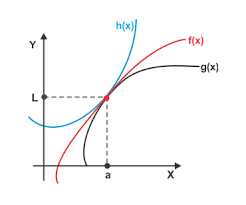
\includegraphics[width=0.6\textwidth]{fig_lim/TeorConfronto}
 \caption{Ilustração do Teorema do Confronto}
  \label{fig:TeorConfronto}
\end{figure}

\noindent { \contour{green}{\color{black}\scshape Desafio:}} Na Seção \ref{sec:LimFundTrig}, mostramos através do uso de tabela que $$\lim_{x\to 0} \frac{\sen x}{x}=1$$
Existem diferentes demonstrações para este limite. Pesquise-as e apresente uma mais convincente possível. Utilizando o limite anterior demonstre que $$\lim_{x\to 0} \frac{\cos x -1}{x}=0$$
\subsection{Exercícios resolvidos}

\begin{exeresol}
  Sabendo que $x^3 \leq f(x) \leq \sqrt{x}$ para $0 < x < 1$, calcule
  \begin{equation*}
    \lim_{x\to 0^+} f(x).
  \end{equation*}
  \begin{resol}
  Pelo Teorema do Confronto, temos
  \begin{equation*}
    \lim_{x\to 0^+} \cancelto{0}{x^3} \leq \lim_{x\to 0^+} f(x) \leq \lim_{x\to 0^+} \cancelto{0}{\sqrt{x}}.
  \end{equation*}
  Logo,
  \begin{equation*}
    \lim_{x\to 0^+} f(x) = 0
  \end{equation*}
\end{resol}
\end{exeresol}


\subsection{Exercícios}

\begin{exer}
  Supondo que $$1-x^2/3 \leq u(x) \leq 1-x^2/2$$ para todo $x\neq 0$, determine  $\lim_{x\to 0} u(x)$.
\end{exer}
\begin{resp}
  $1$
\end{resp}

\begin{exer}
  Calcule
  \begin{multicols}{2}
   \begin{compactenum}[a)]
  \item $ \lim_{x\to \infty} e^{-x}\cos x$\\
  \item $ \lim_{x\to \infty} \frac{2-\cos x}{x+3}$\\
  \item $\lim_{x\to 0} x^2\sin\pc{\frac{1}{x}}$\\
  \item $\lim_{x\to 0} \sqrt{x^3+x^2}\sin\frac{\pi}{x}$
  \end{compactenum}
  \end{multicols}
 
  \end{exer}
\begin{resp}
\begin{multicols}{4}
\begin{compactenum}[a)]
\item $0$
\item  $0$
\item  $0$
\item $0$
\end{compactenum}
\end{multicols}
\end{resp}

\section{Continuidade}\hypertarget{Continuidade}{}\label{sec:Continuidade}
O conceito de continuidade em matemática é o que utilizamos no nosso cotidiano, isto é, continuidade implica numa ligeira variação da função, sem saltos bruscos que desequilibrem o gráfico. Geometricamente, uma função \(f\) é contínua no seu domínio quando seu gráfico não tem quebras ou espaços em nenhum ponto que pertença ao domínio. Isto é, seu gráfico pode ser traçado sem tirar o lápis do papel.

\begin{framed}\begin{definition}
Dizemos que uma {\bf função} $f$ é {\bf contínua} em um ponto $x_0$, quando 
\begin{compactenum}[(i)]
\item $f(x_0)$ está definida;
\item existe o limite $\displaystyle \lim_{x\to x_0} f(x)$ e
\item \begin{equation*}
  \lim_{x\to x_0} f(x) = f(x_0)
\end{equation*}
\end{compactenum}
\end{definition}\end{framed}

 \textcolor{red}{Quando a {\bf função} $f$ não é contínua em um dado ponto $x_0$, dizemos que $f$ é {\bf descontínua} neste ponto.}\\

\vspace{0.2cm}
\begin{ex}\label{ex:conta}
  Consideremos a seguinte função
  \begin{equation*}
    f(x) = \left\{
      \begin{array}{ll}
        \frac{x-2}{(x+1)(x-2)}, & x\neq 2\\
        -4, & x=2
      \end{array}
\right.
\end{equation*}
Na Figura \ref{fig:ex_conta}, temos um esboço do gráfico de $f$.

\begin{figure}[!htb]
  \centering
  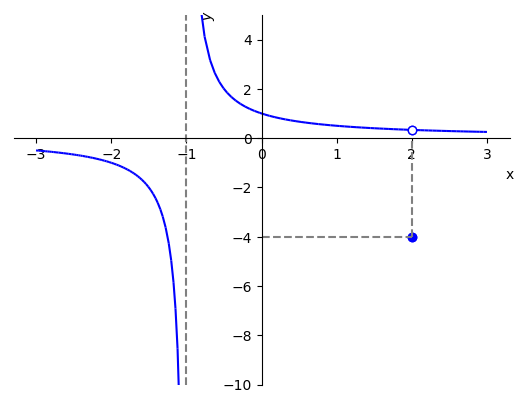
\includegraphics[width=0.6\textwidth]{fig_lim/fig_ex_conta}
  \caption{Esboço do gráfico da função $f$ definida no Exemplo \ref{ex:conta}.}
  \label{fig:ex_conta}
\end{figure}

Vejamos a continuidade desta função nos seguintes pontos:
\begin{enumerate}[a)]
\item $x=-2$. Neste ponto, temos $f(-2) = -1$ e
  \begin{equation*}
    \lim_{x\to -2} \frac{x-2}{(x+1)(x-2)} = \frac{-4}{-1\cdot(-4)} = -1 = f(-2)
  \end{equation*}
  Com isso, concluímos que $f$ é contínua no ponto $x=-2$.
\item $x=-1$. Neste ponto,
  \begin{equation*}
    f(-1) = \frac{(x-2)}{(x+1)(x-2)} = \frac{1}{x-1} = \frac{1}{0}
  \end{equation*}
  logo, f(-1) não está definido e, portanto, $f$ é descontínua neste ponto. Observemos que $f$ tem uma assíntota vertical em $x=-1$, verifique!
\item $x=2$. Neste ponto, temos $f(2)=-4$ e
  \begin{equation*}
    \lim_{x\to 2} \frac{x-2}{(x+1)(x-2)} = \lim_{x\to 2} \frac{1}{x+1} = \frac{1}{3} \neq f(2)
  \end{equation*}
  Portanto, concluímos que $f$ é descontínua em $x=2$.
\end{enumerate}
\end{ex}

\newpage
\nota{
Uma função $f$ é dita ser {\bf contínua em um intervalo} $(a, b)$, quando $f$ é contínua em todos os pontos $x_0\in (a, b)$. Para intervalos, $[a, b)$, $(a, b]$ ou $[a, b]$, empregamos a noção de continuidade lateral nos pontos de extremos fechados dos intervalos. Quando uma função é contínua em $(-\infty, \infty)$, dizemos que ela é {\bf contínua em toda parte}.
}
\begin{ex}\normalfont{(Continuidade da função valor absoluto.)}~
 \\ A função valor absoluto é contínua em toda parte. De fato, ela é definida por
  \begin{equation*}
    |x| = \left\{
      \begin{array}{ll}
        x, & x\geq 0\\
        -x, & x<0
      \end{array}
    \right.
  \end{equation*}
  Veja o esboço do gráfico desta função na Figura \ref{fig:cap_funcao_funabs}.
  
  Observamos que para $x\in(-\infty, 0)$ temos $|x| = -x$ que é contínua para todos estes valores de $x$. Também, para $x\in(0,\infty)$ temos $|x|=x$ que é contínua para todos estes valores de $x$. Agora, em $x=0$, temos $|0|=0$ e
  \begin{align*}
    \lim_{x\to 0^+} |x| &= \lim_{x\to 0^+} x = 0\\
    \lim_{x\to 0^-} |x| &= \lim_{x\to 0^-} -x = 0
  \end{align*}
  Logo,
  \begin{equation*}
    \lim_{x\to 0} |x| = 0 = |0|
  \end{equation*}
  Com tudo isso, concluímos que a função valor absoluto é contínua em toda parte.
\end{ex}

\begin{framed}\begin{prop}\normalfont{(Propriedades de funções contínuas)}
  Se $f$ e $g$ são funções contínuas em $x=c_0$ e $k$ um número real, então também são contínuas em $x=x_0$ as funções:
  \begin{multicols}{2}
  \begin{itemize}
  \item $kf$
  \item $f\pm g$
  \item $f\cdot g$
  \item $f/g$, se $g(x_0)\neq 0$
  \item $f^k$, se existe $f^k(x_0)$.
  \end{itemize}\end{multicols}
\end{prop}\end{framed}

\begin{ex}
  {\bf Polinômios são contínuos em toda parte}. Isto é, se $p(x) = a_nx^n+a_{n-1}x^{n-1}+\cdots+a_1x+a_0$, então
  \begin{equation*}
    \lim_{x\to x_0} p(x) = p(x_0),
  \end{equation*}
  para qualquer $x_0\in\mathbb{R}$. Por exemplo,
  \begin{equation*}
    \lim_{x\to -1} 2 - x^2 + x^5 = 2 - (-1)^2 + (-1)^5 = 0
  \end{equation*}
\end{ex}

\begin{ex}
  {\bf Funções racionais $r(x) = p(x)/q(x)$ são contínuas em todos os pontos de seus domínios}. Por exemplo, a função racional
  \begin{equation*}
    f(x) = \frac{x-1}{x^2-1}
  \end{equation*}
  é descontínua nos pontos
  \begin{equation*}
    x^2-1 = 0 \Rightarrow x = \pm 1,
  \end{equation*}
  pois $f$ não está definida nestes pontos. Agora, para $x_0\neq 1$ e $x_0\neq -1$, temos
  \begin{align*}
    \lim_{x\to x_0} f(x) &= \lim_{x\to x_0} \frac{x-1}{x^2-1}\\
                         &= \frac{x_0-1}{x_0^2-1} = f(x_0)
  \end{align*}
  Por exemplo,
  \begin{equation*}
    \lim_{x\to 0} f(x) = \frac{0-1}{0^2-1} = 1 = f(0)
  \end{equation*}
  Ou seja, $f$ é contínua nos intervalos $(-\infty, -1) \cup (-1, 1) \cup (1, \infty)$, que coincide com seu domínio.
\end{ex}

\nota{
  \textcolor{red}{São contínuas em todo seu domínio as funções potência, polinomiais, racionais, trigonométricas, exponenciais e logarítmicas.}
}

\begin{framed}
\begin{prop}[Composição de funções contínuas]~
\\  Se $f$ é contínua no ponto $x_0$ e $g$ é contínua no ponto $f(x_0)$, então $g\circ f$ é contínua no ponto $x_0$.
\end{prop}\end{framed}

\begin{ex}
  Vejamos os seguintes casos:
  \begin{enumerate}[a)]
  \item $y = \sqrt{x^2-1}$ é descontínua nos pontos $x$ tais que
    \begin{equation*}
      x^2-1<0\Rightarrow -1<x<1
    \end{equation*}
    Isto é, esta função é contínua em $(-\infty,-1]\cup[1,\infty)$.
  \item $\displaystyle y = \left|\frac{x-1}{x^2-1}\right|$ é descontínua nos pontos $x$ tais que
    \begin{equation*}
      x^2-1=0\Rightarrow x=\pm 1
    \end{equation*}
  \end{enumerate}
\end{ex}

\begin{framed}
\begin{teo}[Limite da função composta]~
\\ Sejam $f$ e $g$ duas funções tais que exista a função composta $(g\circ f)(x)$ , isto é,  $(g\circ f)(x) = g( f (x ))$.\\%\marginnote{teste}[-1cm]
Se $\displaystyle\lim_{x\to x_0} f(x)=a$ e $g$ é uma função contínua em $a$, então,$\displaystyle \lim_{x\to x_0} g(f(x))=\lim_{u\to a} g(u)$. 
\end{teo}
\end{framed}
\nota{
  Esse teorema é muito útil e convém notar que, sendo a função $g$ contínua em $a$ e $\displaystyle\lim_{x\to x_0} f(x)=a$, então $\displaystyle\lim_{x\to x_0} g(f(x))=g(a)=g(\lim_{x\to x_0} f(x))$ 
}

\begin{ex}
  Podemos explorar a continuidade para calcularmos limites. Por exemplo,
  \begin{equation*}
    \lim_{x\to 0} \sqrt{x+4}\cdot e^{\sen x} = \sqrt{\lim_{x\to 0} x+4}\cdot e^{\displaystyle\sen \lim_{x\to 0} x} = \sqrt{4}\cdot e^{0} = 2
  \end{equation*}
\end{ex}

\begin{framed}\begin{teo}\normalfont{(Teorema do valor intermediário)}\label{teo:valorintermediario}
\\  Uma função $f$ contínua em um intervalo fechado $[a, b]$, assume todos os valores entre $f(a)$ e $f(b)$.
\end{teo}\end{framed}

\begin{ex}
Verifique que $f(x)=x^3-x-1$ tem (pelo menos) um zero no intervalo $(0, 2)$.\\
\begin{solution}

De fato, $f$ é contínua no intervalo $[0,2]$ e, pelo teorema do valor intermediário, assume todos os valores entre $f(0)=-1<0$ e $f(2)=5>0$. Observemos que $y = 0$ está entre $f(0)$ e $f(2)$. Veja a Figura \ref{fig:cap_lim_ex_teoint}.

  \begin{figure}[htb]
    \centering
    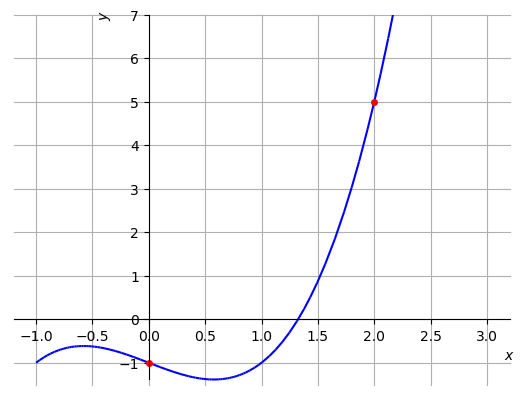
\includegraphics[width=0.7\textwidth]{fig_lim/fig_cap_lim_ex_teoint}
    \caption{Esboço do gráfico da função $f(x) = x^3-x-1$.}
    \label{fig:cap_lim_ex_teoint}
  \end{figure}
\end{solution}
\end{ex}

\subsection{Exercícios resolvidos}

\begin{exeresol}
  Encontre os pontos de continuidade das funções:
  \begin{compactenum}[a)]
  \item $  f(x) = \frac{|x|}{x}$\\
  \begin{resol}
     Observamos que a função é descontínua em $x=0$, pois não está definida neste ponto. Agora, para $x < 0$, temos
  \begin{equation*}
    f(x) = \frac{|x|}{x} = \frac{-x}{x} = -1
  \end{equation*}
  Ou seja, para $x<0$ a função é constante igual a $-1$ e, portanto, contínua.

  Para $x > 0$, temos
  \begin{equation*}
    f(x) = \frac{|x|}{x} = \frac{x}{x} = 1
  \end{equation*}
  I.e., para $x > 0$ a função é constante igual a $1$ e, portanto, contínua.

  Concluímos que $f(x)$ é contínua em $\mathbb{R}\setminus\{0\}$. \dica Faça o esboço do gráfico desta função!
  \end{resol}
  \item $f(x) = \ln\left(\frac{x+1}{x-1}\right)  $\\\\
  \begin{resol}
  A função $f$ pode ser vista como a composição da função logaritmo natural $g(x) = \ln x$ com a função racional $\displaystyle h(x) = \frac{x+1}{x-1}$. Observamos que:
  \begin{enumerate}[a)]
  \item a função logaritmo natural é contínua em todo o seu domínio, i.e. $g$ é contínua para todo $x > 0$;
  \item a função racional $\displaystyle h(x) = \frac{x+1}{x-1}$ é contínua para todo $x\neq 1$.
  \end{enumerate}
  Lembrando que a composição de funções contínuas é contínua, temos que a função $f(x) = g(h(x))$ é contínua nos pontos de continuidade da função $h$ tais que $h(x) > 0$, i.e. para $x\neq 1$ e
  \begin{align*}
    \frac{x+1}{x-1} > 0
  \end{align*}
  Fazendo o estudo de sinal
  \begin{center}
    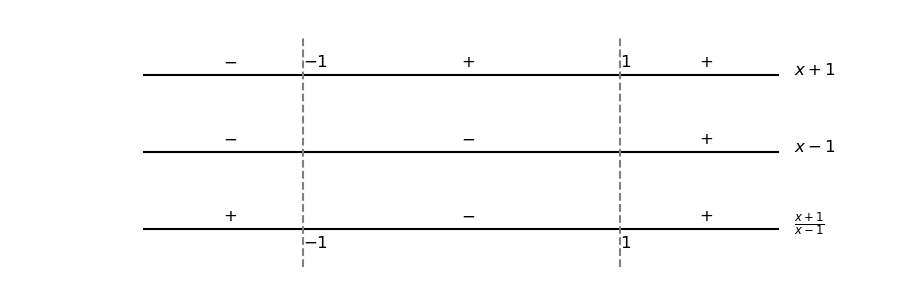
\includegraphics[width=0.8\textwidth]{fig_lim/fig_cap_lim_exeresol_estsinal}
  \end{center}
  vemos que $h(x) > 0$ em $(-\infty, -1)\cup (1, \infty)$.

  Em resumo, $h$ é contínua em $(0, \infty)$ e $g$ é contínua e positiva em $(-\infty, -1)\cup (1, \infty)$. A função $f = (h\circ g)$ é contínua na interseção destes conjuntos, i.e. $f$ é contínua em $(1, \infty)$. 
\end{resol}
  \end{compactenum}
  \end{exeresol}

\subsection{Exercícios}
\begin{exer}
  Encontre os pontos de continuidade das funções
  \begin{multicols}{2}
  \begin{compactenum}[a)]
  \item $f(x) = \frac{x^3 - 27}{x^2 - 3x + 2}$
  \item $ f(x) = \sqrt{\frac{x^3 - 27}{x^2 - 3x + 2}}$
  \end{compactenum}
  \end{multicols}
 \end{exer}
\begin{resp}
\begin{compactenum}[a)]
\item  $\mathbb{R}\setminus\{1,2\}$
\item   $(1, 2)\cup (3, \infty)$
\end{compactenum}
 \end{resp}

\begin{exer}
  Calcule
  \begin{equation*}
    \lim_{x\to \pi} \ln \left(\frac{\sen \frac{x}{2} - \cos x}{2}\right)
  \end{equation*}
\end{exer}
\begin{resp}
  $0$
\end{resp}

\section{Recapitulando}
Neste capítulo, apresentamos o \hyperlink{ConceitoLimite}{conceito de limite} com o intuito de que o aluno entenda a importância do assunto e, assim, dar continuidade ao nosso estudo. 

Nas seções subsequentes, as \hyperlink{PropLimite}{principais propriedades} e leis sobre limites foram apresentadas. Desde que a obtenção de um limite não é sempre direta, isto é, avaliando a função no ponto em questão, a definição de \hyperlink{LimLateral}{limites laterais} foi introduzida.

Cálculo de \hyperlink{Ind0/0}{indeterminações do tipo $\frac{0}{0}$} foram apresentadas e como resolver limites envolvendo-as. Seguidamente foram apresentados os limites fundamentas \hyperlink{LimFundExp}{exponencial} e \hyperlink{LimFundTrig}{trigonométrico}.

Dando continuidade ao nosso estudo, também foram considerados os casos onde o ponto em questão cresce ou decresce ilimitadamente, tal assunto é conhecido como \hyperlink{Lim_no_Inf}{limites ao infinito}. O conceito de \hyperlink{LimInf}{limites infinitos} foi apresentado para definir o fato em que o limite solicitado tende a \(+\infty\), ou \(-\infty\) quanto mais próximo se esteja do ponto em questão.

Desde que essa teoria analisa os pontos onde a função estudada tem um comportamento crítico, foi necessário complementá-la com a introdução da definição das assíntotas \hyperlink{AssintVert}{verticais} e \hyperlink{AssintHoriz}{horizontais}, já que esse conceito estabelece, caso elas existam, o comportamento da função próxima delas.

Diversos exemplos foram apresentados ilustrando todos esses conceitos. Exploramos os conceitos de limites calculados com apoio de desigualdades, com atenção especial ao \hyperlink{TeoConfronto}{Teorema do Confronto}.


A definição de \hyperlink{Continuidade}{continuidade} em intervalos foi apresentada, isto é, envolvendo intervalos da forma: \((a,b)\), \([a,b]\), \([a,b)\) e \((a,b]\). Diversos teoremas foram vistos para nos ajudar a mostrar se uma função é ou não contínua. Mostramos como a continuidade de uma função está relacionada com a sua inversa. Exemplos foram desenvolvidos tentando ilustrar todos esses itens.

Desde que já estudamos limites e continuidade, podemos no próximo capítulo avançar para as noções básicas sobre derivada, conceito muito utilizado para resolver uma ampla gama de problemas, tais como determinação de retas tangentes e valores extremos de uma função dada, entre outras aplicações.
\end{document}
